\documentclass{whiteboard}
\begin{document}
\begin{frame}[plain,t]
\bbcover{OJ 10459}{The Tree Root}{Prof. Edson Alves}{Faculdade UnB Gama}

\end{frame}
\begin{frame}[plain,t]
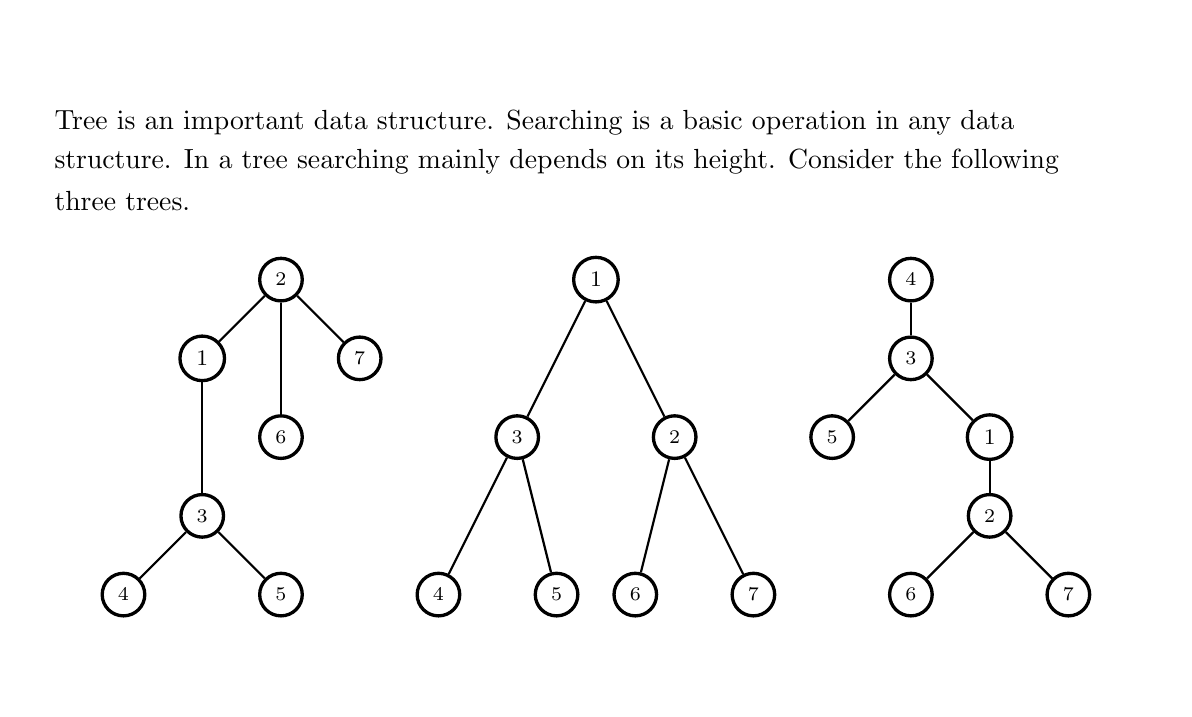
\begin{tikzpicture}
\node[draw,opacity=0] at (0, 0) {x};
\node[draw,opacity=0] at (14, 8) {x};

	\node[anchor=west] (line1) at (0.0, 7.0) { \bbenglish{Tree is an important data structure. Searching is a basic operation in any data} };

	\node[anchor=west] (line2) at (0.0, 6.5) { \bbenglish{structure. In a tree searching mainly depends on its height. Consider the following} };

	\node[anchor=west] (line3) at (0.0, 6.0) { \bbenglish{three trees.} };

	\node[draw,very thick,circle] (a1) at (2.0, 4.0) { \footnotesize \bbtext{1} };

	\node[draw,very thick,circle] (a2) at (3.0, 5.0) { \scriptsize \bbtext{2} };

	\node[draw,very thick,circle] (a3) at (2.0, 2.0) { \scriptsize \bbtext{3} };

	\node[draw,very thick,circle] (a4) at (1.0, 1.0) { \scriptsize \bbtext{4} };

	\node[draw,very thick,circle] (a5) at (3.0, 1.0) { \scriptsize \bbtext{5} };

	\node[draw,very thick,circle] (a6) at (3.0, 3.0) { \scriptsize \bbtext{6} };

	\node[draw,very thick,circle] (a7) at (4.0, 4.0) { \scriptsize \bbtext{7} };

	\draw[thick](a2) to (a1);

	\draw[thick](a2) to (a6);

	\draw[thick](a2) to (a7);

	\draw[thick](a1) to (a3);

	\draw[thick](a3) to (a4);

	\draw[thick](a3) to (a5);

	\node[draw,very thick,circle] (b1) at (7.0, 5.0) { \footnotesize \bbtext{1} };

	\node[draw,very thick,circle] (b2) at (8.0, 3.0) { \scriptsize \bbtext{2} };

	\node[draw,very thick,circle] (b3) at (6.0, 3.0) { \scriptsize \bbtext{3} };

	\node[draw,very thick,circle] (b4) at (5.0, 1.0) { \scriptsize \bbtext{4} };

	\node[draw,very thick,circle] (b5) at (6.5, 1.0) { \scriptsize \bbtext{5} };

	\node[draw,very thick,circle] (b6) at (7.5, 1.0) { \scriptsize \bbtext{6} };

	\node[draw,very thick,circle] (b7) at (9.0, 1.0) { \scriptsize \bbtext{7} };

	\draw[thick](b1) to (b3);

	\draw[thick](b1) to (b2);

	\draw[thick](b2) to (b7);

	\draw[thick](b2) to (b6);

	\draw[thick](b3) to (b4);

	\draw[thick](b3) to (b5);

	\node[draw,very thick,circle] (c1) at (12.0, 3.0) { \footnotesize \bbtext{1} };

	\node[draw,very thick,circle] (c2) at (12.0, 2.0) { \scriptsize \bbtext{2} };

	\node[draw,very thick,circle] (c3) at (11.0, 4.0) { \scriptsize \bbtext{3} };

	\node[draw,very thick,circle] (c4) at (11.0, 5.0) { \scriptsize \bbtext{4} };

	\node[draw,very thick,circle] (c5) at (10.0, 3.0) { \scriptsize \bbtext{5} };

	\node[draw,very thick,circle] (c6) at (11.0, 1.0) { \scriptsize \bbtext{6} };

	\node[draw,very thick,circle] (c7) at (13.0, 1.0) { \scriptsize \bbtext{7} };

	\draw[thick](c4) to (c3);

	\draw[thick](c2) to (c6);

	\draw[thick](c2) to (c7);

	\draw[thick](c1) to (c2);

	\draw[thick](c3) to (c1);

	\draw[thick](c3) to (c5);

\end{tikzpicture}
\end{frame}
\begin{frame}[plain,t]
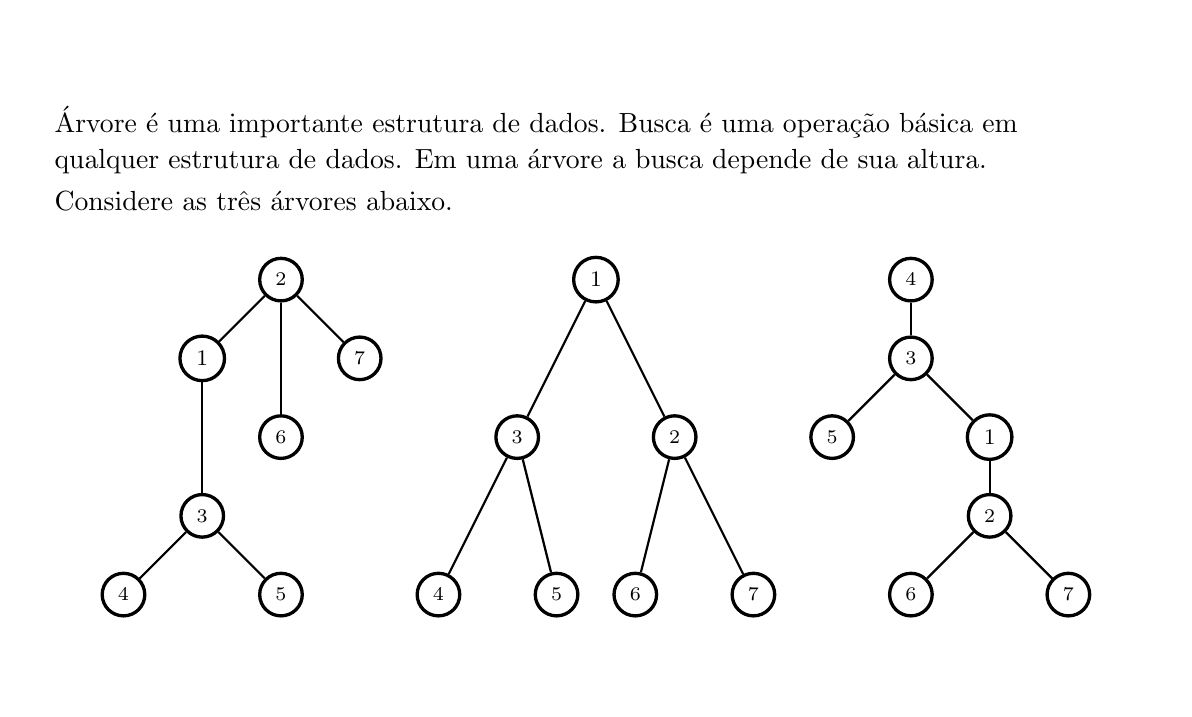
\begin{tikzpicture}
\node[draw,opacity=0] at (0, 0) {x};
\node[draw,opacity=0] at (14, 8) {x};

	\node[anchor=west] (line1) at (0.0, 7.0) { \bbtext{Árvore é uma importante estrutura de dados. Busca é uma operação básica em} };

	\node[anchor=west] (line2) at (0.0, 6.5) { \bbtext{qualquer estrutura de dados. Em uma árvore a busca depende de sua altura. } };

	\node[anchor=west] (line3) at (0.0, 6.0) { \bbtext{Considere as três árvores abaixo.} };

	\node[draw,very thick,circle] (a1) at (2.0, 4.0) { \footnotesize \bbtext{1} };

	\node[draw,very thick,circle] (a2) at (3.0, 5.0) { \scriptsize \bbtext{2} };

	\node[draw,very thick,circle] (a3) at (2.0, 2.0) { \scriptsize \bbtext{3} };

	\node[draw,very thick,circle] (a4) at (1.0, 1.0) { \scriptsize \bbtext{4} };

	\node[draw,very thick,circle] (a5) at (3.0, 1.0) { \scriptsize \bbtext{5} };

	\node[draw,very thick,circle] (a6) at (3.0, 3.0) { \scriptsize \bbtext{6} };

	\node[draw,very thick,circle] (a7) at (4.0, 4.0) { \scriptsize \bbtext{7} };

	\draw[thick](a2) to (a1);

	\draw[thick](a2) to (a6);

	\draw[thick](a2) to (a7);

	\draw[thick](a1) to (a3);

	\draw[thick](a3) to (a4);

	\draw[thick](a3) to (a5);

	\node[draw,very thick,circle] (b1) at (7.0, 5.0) { \footnotesize \bbtext{1} };

	\node[draw,very thick,circle] (b2) at (8.0, 3.0) { \scriptsize \bbtext{2} };

	\node[draw,very thick,circle] (b3) at (6.0, 3.0) { \scriptsize \bbtext{3} };

	\node[draw,very thick,circle] (b4) at (5.0, 1.0) { \scriptsize \bbtext{4} };

	\node[draw,very thick,circle] (b5) at (6.5, 1.0) { \scriptsize \bbtext{5} };

	\node[draw,very thick,circle] (b6) at (7.5, 1.0) { \scriptsize \bbtext{6} };

	\node[draw,very thick,circle] (b7) at (9.0, 1.0) { \scriptsize \bbtext{7} };

	\draw[thick](b1) to (b3);

	\draw[thick](b1) to (b2);

	\draw[thick](b2) to (b7);

	\draw[thick](b2) to (b6);

	\draw[thick](b3) to (b4);

	\draw[thick](b3) to (b5);

	\node[draw,very thick,circle] (c1) at (12.0, 3.0) { \footnotesize \bbtext{1} };

	\node[draw,very thick,circle] (c2) at (12.0, 2.0) { \scriptsize \bbtext{2} };

	\node[draw,very thick,circle] (c3) at (11.0, 4.0) { \scriptsize \bbtext{3} };

	\node[draw,very thick,circle] (c4) at (11.0, 5.0) { \scriptsize \bbtext{4} };

	\node[draw,very thick,circle] (c5) at (10.0, 3.0) { \scriptsize \bbtext{5} };

	\node[draw,very thick,circle] (c6) at (11.0, 1.0) { \scriptsize \bbtext{6} };

	\node[draw,very thick,circle] (c7) at (13.0, 1.0) { \scriptsize \bbtext{7} };

	\draw[thick](c4) to (c3);

	\draw[thick](c2) to (c6);

	\draw[thick](c2) to (c7);

	\draw[thick](c1) to (c2);

	\draw[thick](c3) to (c1);

	\draw[thick](c3) to (c5);

\end{tikzpicture}
\end{frame}
\begin{frame}[plain,t]
\vspace*{\fill}

\bbenglish{If you observe carefully, you will see that all trees are same except different nodes are used as roots.  Here the height of the tree varies with the selection of the root. In the 1st tree root is `\texttt{2}' and height is $3$. In 2nd one root is `\texttt{1}' and height is $2$. And in last one root is `\texttt{4}' and height is $4$. We will call `\texttt{1}' best root as it keeps the tree with the least possible height and `\texttt{4}' worst root for the opposite reason.}

\vspace{0.1in}

\bbenglish{In this problem, you have to find out all best roots and worst roots for a given tree.}

\vspace*{\fill}
\end{frame}
\begin{frame}[plain,t]
\vspace*{\fill}

\bbtext{Se você observar atentamente, você verá que todas as três árvores são idênticas, exceto pelo fato de terem escolhidos nós diferentes como raízes.  Aqui a altura da árvore varia de acordo com a escolha da raiz. Na primeira árvore a raiz é `\texttt{2}' e a altura é $3$. Na segunda a raiz é `\texttt{1}' e a altura é $2$. E na última a raiz é `\texttt{4}' e a altura é $4$. Nos dizemos que `\texttt{1}' é uma raiz ótima no sentido que ela minimiza a altura máxima e `\texttt{4}' uma raiz péssima pela razão oposta.}

\vspace{0.1in}

\bbtext{Neste problema você deve encontrar todas as raízes ótimas e péssimas de uma dada árvore.}

\vspace*{\fill}
\end{frame}
\begin{frame}[plain,t]
\vspace*{\fill}

\bbbold{Input}

\vspace{0.1in}

\bbenglish{Each dataset starts with a positive integer $N$ $(3\leq N\leq 5000)$, which is the number of nodes in the tree. Each node in the tree has a unique id from $1$ to $N$. Then successively for each $i$’th node there will be a positive integer $K[i]$ following id of $K[i]$ nodes which are adjacent to $i$. Input is terminated by \texttt{EOF}.}

\vspace{0.2in}

\bbbold{Output}

\vspace{0.1in}

\bbenglish{For each dataset print two lines. In the 1st line show all the best roots in ascending order and in next line show all worst roots in ascending order. See sample output for exact format.}

\vspace*{\fill}
\end{frame}
\begin{frame}[plain,t]
\vspace*{\fill}

\bbbold{Entrada}

\vspace{0.1in}

\bbtext{Cada caso de teste começa com um inteiro positivo $N$ $(3\leq N\leq 5000)$, o qual indica o número de nós na árvore. Cada nó da árvore tem um identificador único no intervalo de $1$ a $N$. Então para cada $i$-ésimo nó haverá um inteiro positivo $K[i]$ seguido pelos identificadores dos $K[i]$ nós adjacentes a $i$. A entrada termina com \texttt{EOF}.}

\vspace{0.2in}

\bbbold{Output}

\vspace{0.1in}

\bbtext{Para cada caso de teste imprima duas linhas. Na primeira linha mostre todas as raízes ótimas, em ordem crescente, e na linha seguinte todas as raízes péssimas, em ordem crescente. Veja o exemplo para o formato exato da saída.}

\vspace*{\fill}
\end{frame}
\begin{frame}[plain,t]
\begin{tikzpicture}
\node[draw,opacity=0] at (0, 0) {x};
\node[draw,opacity=0] at (14, 8) {x};

	\node[anchor=west] (header) at (0, 7.0) { \bbbold{Exemplo de entrada e saída} };

\end{tikzpicture}
\end{frame}
\begin{frame}[plain,t]
\begin{tikzpicture}
\node[draw,opacity=0] at (0, 0) {x};
\node[draw,opacity=0] at (14, 8) {x};

	\node[anchor=west] (header) at (0, 7.0) { \bbbold{Exemplo de entrada e saída} };


	\node[anchor=west] (line1) at (1.0, 6.0) { \bbtext{\texttt{7} } };

\end{tikzpicture}
\end{frame}
\begin{frame}[plain,t]
\begin{tikzpicture}
\node[draw,opacity=0] at (0, 0) {x};
\node[draw,opacity=0] at (14, 8) {x};

	\node[anchor=west] (header) at (0, 7.0) { \bbbold{Exemplo de entrada e saída} };


	\node[anchor=west] (line1) at (1.0, 6.0) { \bbtext{\texttt{7} } };


	\draw[->,color=BBViolet] (1.25, 5.0) to  (1.25, 5.75);

	\node[] (r) at (1.25, 4.75) { \footnotesize \bbcomment{\# número de nós} };

\end{tikzpicture}
\end{frame}
\begin{frame}[plain,t]
\begin{tikzpicture}
\node[draw,opacity=0] at (0, 0) {x};
\node[draw,opacity=0] at (14, 8) {x};

	\node[anchor=west] (header) at (0, 7.0) { \bbbold{Exemplo de entrada e saída} };


	\node[anchor=west] (line1) at (1.0, 6.0) { \bbtext{\texttt{7} } };





	\node[draw,very thick,circle] (node1) at (7.0, 4.0) { \bbtext{1} };

	\node[draw,very thick,circle] (node2) at (9.0, 7.0) { \bbtext{2} };

	\node[draw,very thick,circle] (node3) at (11.0, 7.0) { \bbtext{3} };

	\node[draw,very thick,circle] (node4) at (13.0, 5.0) { \bbtext{4} };

	\node[draw,very thick,circle] (node5) at (13.0, 3.0) { \bbtext{5} };

	\node[draw,very thick,circle] (node6) at (11.0, 1.0) { \bbtext{6} };

	\node[draw,very thick,circle] (node7) at (9.0, 1.0) { \bbtext{7} };

\end{tikzpicture}
\end{frame}
\begin{frame}[plain,t]
\begin{tikzpicture}
\node[draw,opacity=0] at (0, 0) {x};
\node[draw,opacity=0] at (14, 8) {x};

	\node[anchor=west] (header) at (0, 7.0) { \bbbold{Exemplo de entrada e saída} };


	\node[anchor=west] (line1) at (1.0, 6.0) { \bbtext{\texttt{7} } };





	\node[draw,very thick,circle] (node1) at (7.0, 4.0) { \bbtext{1} };

	\node[draw,very thick,circle] (node2) at (9.0, 7.0) { \bbtext{2} };

	\node[draw,very thick,circle] (node3) at (11.0, 7.0) { \bbtext{3} };

	\node[draw,very thick,circle] (node4) at (13.0, 5.0) { \bbtext{4} };

	\node[draw,very thick,circle] (node5) at (13.0, 3.0) { \bbtext{5} };

	\node[draw,very thick,circle] (node6) at (11.0, 1.0) { \bbtext{6} };

	\node[draw,very thick,circle] (node7) at (9.0, 1.0) { \bbtext{7} };


	\node[anchor=west] (line2) at (1.0, 5.5) { \bbtext{\texttt{2 2 3} } };

\end{tikzpicture}
\end{frame}
\begin{frame}[plain,t]
\begin{tikzpicture}
\node[draw,opacity=0] at (0, 0) {x};
\node[draw,opacity=0] at (14, 8) {x};

	\node[anchor=west] (header) at (0, 7.0) { \bbbold{Exemplo de entrada e saída} };


	\node[anchor=west] (line1) at (1.0, 6.0) { \bbtext{\texttt{7} } };


	\draw[->,color=BBViolet] (1.25, 5.25) to  (1.25, 4.25);

	\node[] (r) at (1.25, 4.0) { \footnotesize $K_1$ };


	\node[draw,very thick,circle] (node1) at (7.0, 4.0) { \bbtext{1} };

	\node[draw,very thick,circle] (node2) at (9.0, 7.0) { \bbtext{2} };

	\node[draw,very thick,circle] (node3) at (11.0, 7.0) { \bbtext{3} };

	\node[draw,very thick,circle] (node4) at (13.0, 5.0) { \bbtext{4} };

	\node[draw,very thick,circle] (node5) at (13.0, 3.0) { \bbtext{5} };

	\node[draw,very thick,circle] (node6) at (11.0, 1.0) { \bbtext{6} };

	\node[draw,very thick,circle] (node7) at (9.0, 1.0) { \bbtext{7} };


	\node[anchor=west] (line2) at (1.0, 5.5) { \bbtext{\texttt{2 2 3} } };




\end{tikzpicture}
\end{frame}
\begin{frame}[plain,t]
\begin{tikzpicture}
\node[draw,opacity=0] at (0, 0) {x};
\node[draw,opacity=0] at (14, 8) {x};

	\node[anchor=west] (header) at (0, 7.0) { \bbbold{Exemplo de entrada e saída} };


	\node[anchor=west] (line1) at (1.0, 6.0) { \bbtext{\texttt{7} } };


	\draw[->,color=BBViolet] (1.65, 5.25) to  (1.65, 4.25);

	\node[] (r) at (1.65, 4.0) { \footnotesize $v_1$ };


	\node[draw,very thick,circle] (node1) at (7.0, 4.0) { \bbtext{1} };

	\node[draw,very thick,circle] (node2) at (9.0, 7.0) { \bbtext{2} };

	\node[draw,very thick,circle] (node3) at (11.0, 7.0) { \bbtext{3} };

	\node[draw,very thick,circle] (node4) at (13.0, 5.0) { \bbtext{4} };

	\node[draw,very thick,circle] (node5) at (13.0, 3.0) { \bbtext{5} };

	\node[draw,very thick,circle] (node6) at (11.0, 1.0) { \bbtext{6} };

	\node[draw,very thick,circle] (node7) at (9.0, 1.0) { \bbtext{7} };


	\node[anchor=west] (line2) at (1.0, 5.5) { \bbtext{\texttt{2 2 3} } };







\end{tikzpicture}
\end{frame}
\begin{frame}[plain,t]
\begin{tikzpicture}
\node[draw,opacity=0] at (0, 0) {x};
\node[draw,opacity=0] at (14, 8) {x};

	\node[anchor=west] (header) at (0, 7.0) { \bbbold{Exemplo de entrada e saída} };


	\node[anchor=west] (line1) at (1.0, 6.0) { \bbtext{\texttt{7} } };





	\node[draw,very thick,circle] (node1) at (7.0, 4.0) { \bbtext{1} };

	\node[draw,very thick,circle] (node2) at (9.0, 7.0) { \bbtext{2} };

	\node[draw,very thick,circle] (node3) at (11.0, 7.0) { \bbtext{3} };

	\node[draw,very thick,circle] (node4) at (13.0, 5.0) { \bbtext{4} };

	\node[draw,very thick,circle] (node5) at (13.0, 3.0) { \bbtext{5} };

	\node[draw,very thick,circle] (node6) at (11.0, 1.0) { \bbtext{6} };

	\node[draw,very thick,circle] (node7) at (9.0, 1.0) { \bbtext{7} };


	\node[anchor=west] (line2) at (1.0, 5.5) { \bbtext{\texttt{2 2 3} } };








	\draw[thick](node1) to (node2);


\end{tikzpicture}
\end{frame}
\begin{frame}[plain,t]
\begin{tikzpicture}
\node[draw,opacity=0] at (0, 0) {x};
\node[draw,opacity=0] at (14, 8) {x};

	\node[anchor=west] (header) at (0, 7.0) { \bbbold{Exemplo de entrada e saída} };


	\node[anchor=west] (line1) at (1.0, 6.0) { \bbtext{\texttt{7} } };


	\draw[->,color=BBViolet] (2.05, 5.25) to  (2.05, 4.25);

	\node[] (r) at (2.05, 4.0) { \footnotesize $v_2$ };


	\node[draw,very thick,circle] (node1) at (7.0, 4.0) { \bbtext{1} };

	\node[draw,very thick,circle] (node2) at (9.0, 7.0) { \bbtext{2} };

	\node[draw,very thick,circle] (node3) at (11.0, 7.0) { \bbtext{3} };

	\node[draw,very thick,circle] (node4) at (13.0, 5.0) { \bbtext{4} };

	\node[draw,very thick,circle] (node5) at (13.0, 3.0) { \bbtext{5} };

	\node[draw,very thick,circle] (node6) at (11.0, 1.0) { \bbtext{6} };

	\node[draw,very thick,circle] (node7) at (9.0, 1.0) { \bbtext{7} };


	\node[anchor=west] (line2) at (1.0, 5.5) { \bbtext{\texttt{2 2 3} } };








	\draw[thick](node1) to (node2);




\end{tikzpicture}
\end{frame}
\begin{frame}[plain,t]
\begin{tikzpicture}
\node[draw,opacity=0] at (0, 0) {x};
\node[draw,opacity=0] at (14, 8) {x};

	\node[anchor=west] (header) at (0, 7.0) { \bbbold{Exemplo de entrada e saída} };


	\node[anchor=west] (line1) at (1.0, 6.0) { \bbtext{\texttt{7} } };





	\node[draw,very thick,circle] (node1) at (7.0, 4.0) { \bbtext{1} };

	\node[draw,very thick,circle] (node2) at (9.0, 7.0) { \bbtext{2} };

	\node[draw,very thick,circle] (node3) at (11.0, 7.0) { \bbtext{3} };

	\node[draw,very thick,circle] (node4) at (13.0, 5.0) { \bbtext{4} };

	\node[draw,very thick,circle] (node5) at (13.0, 3.0) { \bbtext{5} };

	\node[draw,very thick,circle] (node6) at (11.0, 1.0) { \bbtext{6} };

	\node[draw,very thick,circle] (node7) at (9.0, 1.0) { \bbtext{7} };


	\node[anchor=west] (line2) at (1.0, 5.5) { \bbtext{\texttt{2 2 3} } };








	\draw[thick](node1) to (node2);





	\draw[thick](node1) to (node3);

\end{tikzpicture}
\end{frame}
\begin{frame}[plain,t]
\begin{tikzpicture}
\node[draw,opacity=0] at (0, 0) {x};
\node[draw,opacity=0] at (14, 8) {x};

	\node[anchor=west] (header) at (0, 7.0) { \bbbold{Exemplo de entrada e saída} };


	\node[anchor=west] (line1) at (1.0, 6.0) { \bbtext{\texttt{7} } };





	\node[draw,very thick,circle] (node1) at (7.0, 4.0) { \bbtext{1} };

	\node[draw,very thick,circle] (node2) at (9.0, 7.0) { \bbtext{2} };

	\node[draw,very thick,circle] (node3) at (11.0, 7.0) { \bbtext{3} };

	\node[draw,very thick,circle] (node4) at (13.0, 5.0) { \bbtext{4} };

	\node[draw,very thick,circle] (node5) at (13.0, 3.0) { \bbtext{5} };

	\node[draw,very thick,circle] (node6) at (11.0, 1.0) { \bbtext{6} };

	\node[draw,very thick,circle] (node7) at (9.0, 1.0) { \bbtext{7} };


	\node[anchor=west] (line2) at (1.0, 5.5) { \bbtext{\texttt{2 2 3} } };








	\draw[thick](node1) to (node2);





	\draw[thick](node1) to (node3);


	\node[anchor=west] (line3) at (1.0, 5.0) { \bbtext{\texttt{3 1 6 7} } };

\end{tikzpicture}
\end{frame}
\begin{frame}[plain,t]
\begin{tikzpicture}
\node[draw,opacity=0] at (0, 0) {x};
\node[draw,opacity=0] at (14, 8) {x};

	\node[anchor=west] (header) at (0, 7.0) { \bbbold{Exemplo de entrada e saída} };


	\node[anchor=west] (line1) at (1.0, 6.0) { \bbtext{\texttt{7} } };





	\node[draw,very thick,circle] (node1) at (7.0, 4.0) { \bbtext{1} };

	\node[draw,very thick,circle] (node2) at (9.0, 7.0) { \bbtext{2} };

	\node[draw,very thick,circle] (node3) at (11.0, 7.0) { \bbtext{3} };

	\node[draw,very thick,circle] (node4) at (13.0, 5.0) { \bbtext{4} };

	\node[draw,very thick,circle] (node5) at (13.0, 3.0) { \bbtext{5} };

	\node[draw,very thick,circle] (node6) at (11.0, 1.0) { \bbtext{6} };

	\node[draw,very thick,circle] (node7) at (9.0, 1.0) { \bbtext{7} };


	\node[anchor=west] (line2) at (1.0, 5.5) { \bbtext{\texttt{2 2 3} } };








	\draw[thick](node1) to (node2);





	\draw[thick](node1) to (node3);


	\node[anchor=west] (line3) at (1.0, 5.0) { \bbtext{\texttt{3 1 6 7} } };


	\draw[thick](node2) to (node6);

	\draw[thick](node2) to (node7);

\end{tikzpicture}
\end{frame}
\begin{frame}[plain,t]
\begin{tikzpicture}
\node[draw,opacity=0] at (0, 0) {x};
\node[draw,opacity=0] at (14, 8) {x};

	\node[anchor=west] (header) at (0, 7.0) { \bbbold{Exemplo de entrada e saída} };


	\node[anchor=west] (line1) at (1.0, 6.0) { \bbtext{\texttt{7} } };





	\node[draw,very thick,circle] (node1) at (7.0, 4.0) { \bbtext{1} };

	\node[draw,very thick,circle] (node2) at (9.0, 7.0) { \bbtext{2} };

	\node[draw,very thick,circle] (node3) at (11.0, 7.0) { \bbtext{3} };

	\node[draw,very thick,circle] (node4) at (13.0, 5.0) { \bbtext{4} };

	\node[draw,very thick,circle] (node5) at (13.0, 3.0) { \bbtext{5} };

	\node[draw,very thick,circle] (node6) at (11.0, 1.0) { \bbtext{6} };

	\node[draw,very thick,circle] (node7) at (9.0, 1.0) { \bbtext{7} };


	\node[anchor=west] (line2) at (1.0, 5.5) { \bbtext{\texttt{2 2 3} } };








	\draw[thick](node1) to (node2);





	\draw[thick](node1) to (node3);


	\node[anchor=west] (line3) at (1.0, 5.0) { \bbtext{\texttt{3 1 6 7} } };


	\draw[thick](node2) to (node6);

	\draw[thick](node2) to (node7);


	\node[anchor=west] (line4) at (1.0, 4.5) { \bbtext{\texttt{3 1 4 5} } };

\end{tikzpicture}
\end{frame}
\begin{frame}[plain,t]
\begin{tikzpicture}
\node[draw,opacity=0] at (0, 0) {x};
\node[draw,opacity=0] at (14, 8) {x};

	\node[anchor=west] (header) at (0, 7.0) { \bbbold{Exemplo de entrada e saída} };


	\node[anchor=west] (line1) at (1.0, 6.0) { \bbtext{\texttt{7} } };





	\node[draw,very thick,circle] (node1) at (7.0, 4.0) { \bbtext{1} };

	\node[draw,very thick,circle] (node2) at (9.0, 7.0) { \bbtext{2} };

	\node[draw,very thick,circle] (node3) at (11.0, 7.0) { \bbtext{3} };

	\node[draw,very thick,circle] (node4) at (13.0, 5.0) { \bbtext{4} };

	\node[draw,very thick,circle] (node5) at (13.0, 3.0) { \bbtext{5} };

	\node[draw,very thick,circle] (node6) at (11.0, 1.0) { \bbtext{6} };

	\node[draw,very thick,circle] (node7) at (9.0, 1.0) { \bbtext{7} };


	\node[anchor=west] (line2) at (1.0, 5.5) { \bbtext{\texttt{2 2 3} } };








	\draw[thick](node1) to (node2);





	\draw[thick](node1) to (node3);


	\node[anchor=west] (line3) at (1.0, 5.0) { \bbtext{\texttt{3 1 6 7} } };


	\draw[thick](node2) to (node6);

	\draw[thick](node2) to (node7);


	\node[anchor=west] (line4) at (1.0, 4.5) { \bbtext{\texttt{3 1 4 5} } };


	\draw[thick](node3) to (node4);

	\draw[thick](node3) to (node5);

\end{tikzpicture}
\end{frame}
\begin{frame}[plain,t]
\begin{tikzpicture}
\node[draw,opacity=0] at (0, 0) {x};
\node[draw,opacity=0] at (14, 8) {x};

	\node[anchor=west] (header) at (0, 7.0) { \bbbold{Exemplo de entrada e saída} };


	\node[anchor=west] (line1) at (1.0, 6.0) { \bbtext{\texttt{7} } };





	\node[draw,very thick,circle] (node1) at (7.0, 4.0) { \bbtext{1} };

	\node[draw,very thick,circle] (node2) at (9.0, 7.0) { \bbtext{2} };

	\node[draw,very thick,circle] (node3) at (11.0, 7.0) { \bbtext{3} };

	\node[draw,very thick,circle] (node4) at (13.0, 5.0) { \bbtext{4} };

	\node[draw,very thick,circle] (node5) at (13.0, 3.0) { \bbtext{5} };

	\node[draw,very thick,circle] (node6) at (11.0, 1.0) { \bbtext{6} };

	\node[draw,very thick,circle] (node7) at (9.0, 1.0) { \bbtext{7} };


	\node[anchor=west] (line2) at (1.0, 5.5) { \bbtext{\texttt{2 2 3} } };








	\draw[thick](node1) to (node2);





	\draw[thick](node1) to (node3);


	\node[anchor=west] (line3) at (1.0, 5.0) { \bbtext{\texttt{3 1 6 7} } };


	\draw[thick](node2) to (node6);

	\draw[thick](node2) to (node7);


	\node[anchor=west] (line4) at (1.0, 4.5) { \bbtext{\texttt{3 1 4 5} } };


	\draw[thick](node3) to (node4);

	\draw[thick](node3) to (node5);


	\node[anchor=west] (line5) at (1.0, 4.0) { \bbtext{\texttt{1 3} } };
\end{tikzpicture}
\end{frame}
\begin{frame}[plain,t]
\begin{tikzpicture}
\node[draw,opacity=0] at (0, 0) {x};
\node[draw,opacity=0] at (14, 8) {x};

	\node[anchor=west] (header) at (0, 7.0) { \bbbold{Exemplo de entrada e saída} };


	\node[anchor=west] (line1) at (1.0, 6.0) { \bbtext{\texttt{7} } };





	\node[draw,very thick,circle] (node1) at (7.0, 4.0) { \bbtext{1} };

	\node[draw,very thick,circle] (node2) at (9.0, 7.0) { \bbtext{2} };

	\node[draw,very thick,circle] (node3) at (11.0, 7.0) { \bbtext{3} };

	\node[draw,very thick,circle] (node4) at (13.0, 5.0) { \bbtext{4} };

	\node[draw,very thick,circle] (node5) at (13.0, 3.0) { \bbtext{5} };

	\node[draw,very thick,circle] (node6) at (11.0, 1.0) { \bbtext{6} };

	\node[draw,very thick,circle] (node7) at (9.0, 1.0) { \bbtext{7} };


	\node[anchor=west] (line2) at (1.0, 5.5) { \bbtext{\texttt{2 2 3} } };








	\draw[thick](node1) to (node2);





	\draw[thick](node1) to (node3);


	\node[anchor=west] (line3) at (1.0, 5.0) { \bbtext{\texttt{3 1 6 7} } };


	\draw[thick](node2) to (node6);

	\draw[thick](node2) to (node7);


	\node[anchor=west] (line4) at (1.0, 4.5) { \bbtext{\texttt{3 1 4 5} } };


	\draw[thick](node3) to (node4);

	\draw[thick](node3) to (node5);


	\node[anchor=west] (line5) at (1.0, 4.0) { \bbtext{\texttt{1 3} } };

	\node[anchor=west] (line6) at (1.0, 3.5) { \bbtext{\texttt{1 3} } };

\end{tikzpicture}
\end{frame}
\begin{frame}[plain,t]
\begin{tikzpicture}
\node[draw,opacity=0] at (0, 0) {x};
\node[draw,opacity=0] at (14, 8) {x};

	\node[anchor=west] (header) at (0, 7.0) { \bbbold{Exemplo de entrada e saída} };


	\node[anchor=west] (line1) at (1.0, 6.0) { \bbtext{\texttt{7} } };





	\node[draw,very thick,circle] (node1) at (7.0, 4.0) { \bbtext{1} };

	\node[draw,very thick,circle] (node2) at (9.0, 7.0) { \bbtext{2} };

	\node[draw,very thick,circle] (node3) at (11.0, 7.0) { \bbtext{3} };

	\node[draw,very thick,circle] (node4) at (13.0, 5.0) { \bbtext{4} };

	\node[draw,very thick,circle] (node5) at (13.0, 3.0) { \bbtext{5} };

	\node[draw,very thick,circle] (node6) at (11.0, 1.0) { \bbtext{6} };

	\node[draw,very thick,circle] (node7) at (9.0, 1.0) { \bbtext{7} };


	\node[anchor=west] (line2) at (1.0, 5.5) { \bbtext{\texttt{2 2 3} } };








	\draw[thick](node1) to (node2);





	\draw[thick](node1) to (node3);


	\node[anchor=west] (line3) at (1.0, 5.0) { \bbtext{\texttt{3 1 6 7} } };


	\draw[thick](node2) to (node6);

	\draw[thick](node2) to (node7);


	\node[anchor=west] (line4) at (1.0, 4.5) { \bbtext{\texttt{3 1 4 5} } };


	\draw[thick](node3) to (node4);

	\draw[thick](node3) to (node5);


	\node[anchor=west] (line5) at (1.0, 4.0) { \bbtext{\texttt{1 3} } };

	\node[anchor=west] (line6) at (1.0, 3.5) { \bbtext{\texttt{1 3} } };


	\node[anchor=west] (line7) at (1.0, 3.0) { \bbtext{\texttt{1 2} } };

\end{tikzpicture}
\end{frame}
\begin{frame}[plain,t]
\begin{tikzpicture}
\node[draw,opacity=0] at (0, 0) {x};
\node[draw,opacity=0] at (14, 8) {x};

	\node[anchor=west] (header) at (0, 7.0) { \bbbold{Exemplo de entrada e saída} };


	\node[anchor=west] (line1) at (1.0, 6.0) { \bbtext{\texttt{7} } };





	\node[draw,very thick,circle] (node1) at (7.0, 4.0) { \bbtext{1} };

	\node[draw,very thick,circle] (node2) at (9.0, 7.0) { \bbtext{2} };

	\node[draw,very thick,circle] (node3) at (11.0, 7.0) { \bbtext{3} };

	\node[draw,very thick,circle] (node4) at (13.0, 5.0) { \bbtext{4} };

	\node[draw,very thick,circle] (node5) at (13.0, 3.0) { \bbtext{5} };

	\node[draw,very thick,circle] (node6) at (11.0, 1.0) { \bbtext{6} };

	\node[draw,very thick,circle] (node7) at (9.0, 1.0) { \bbtext{7} };


	\node[anchor=west] (line2) at (1.0, 5.5) { \bbtext{\texttt{2 2 3} } };








	\draw[thick](node1) to (node2);





	\draw[thick](node1) to (node3);


	\node[anchor=west] (line3) at (1.0, 5.0) { \bbtext{\texttt{3 1 6 7} } };


	\draw[thick](node2) to (node6);

	\draw[thick](node2) to (node7);


	\node[anchor=west] (line4) at (1.0, 4.5) { \bbtext{\texttt{3 1 4 5} } };


	\draw[thick](node3) to (node4);

	\draw[thick](node3) to (node5);


	\node[anchor=west] (line5) at (1.0, 4.0) { \bbtext{\texttt{1 3} } };

	\node[anchor=west] (line6) at (1.0, 3.5) { \bbtext{\texttt{1 3} } };


	\node[anchor=west] (line7) at (1.0, 3.0) { \bbtext{\texttt{1 2} } };


	\node[anchor=west] (line8) at (1.0, 2.5) { \bbtext{\texttt{1 2} } };

\end{tikzpicture}
\end{frame}
\begin{frame}[plain,t]
\begin{tikzpicture}
\node[draw,opacity=0] at (0, 0) {x};
\node[draw,opacity=0] at (14, 8) {x};

	\node[anchor=west] (header) at (0, 7.0) { \bbbold{Exemplo de entrada e saída} };


	\node[anchor=west] (line1) at (1.0, 6.0) { \bbtext{\texttt{7} } };





	\node[draw,very thick,circle] (node1) at (10.0, 7.0) { \bbtext{1} };

	\node[draw,very thick,circle] (node2) at (12.0, 4.0) { \bbtext{2} };

	\node[draw,very thick,circle] (node3) at (8.0, 4.0) { \bbtext{3} };

	\node[draw,very thick,circle] (node4) at (7.0, 1.0) { \bbtext{4} };

	\node[draw,very thick,circle] (node5) at (9.0, 1.0) { \bbtext{5} };

	\node[draw,very thick,circle] (node6) at (11.0, 1.0) { \bbtext{6} };

	\node[draw,very thick,circle] (node7) at (13.0, 1.0) { \bbtext{7} };


	\node[anchor=west] (line2) at (1.0, 5.5) { \bbtext{\texttt{2 2 3} } };








	\draw[thick](node1) to (node2);





	\draw[thick](node1) to (node3);


	\node[anchor=west] (line3) at (1.0, 5.0) { \bbtext{\texttt{3 1 6 7} } };


	\draw[thick](node2) to (node6);

	\draw[thick](node2) to (node7);


	\node[anchor=west] (line4) at (1.0, 4.5) { \bbtext{\texttt{3 1 4 5} } };


	\draw[thick](node3) to (node4);

	\draw[thick](node3) to (node5);


	\node[anchor=west] (line5) at (1.0, 4.0) { \bbtext{\texttt{1 3} } };

	\node[anchor=west] (line6) at (1.0, 3.5) { \bbtext{\texttt{1 3} } };


	\node[anchor=west] (line7) at (1.0, 3.0) { \bbtext{\texttt{1 2} } };


	\node[anchor=west] (line8) at (1.0, 2.5) { \bbtext{\texttt{1 2} } };









\end{tikzpicture}
\end{frame}
\begin{frame}[plain,t]
\begin{tikzpicture}
\node[draw,opacity=0] at (0, 0) {x};
\node[draw,opacity=0] at (14, 8) {x};

	\node[anchor=west] (header) at (0, 7.0) { \bbbold{Exemplo de entrada e saída} };


	\node[anchor=west] (line1) at (1.0, 6.0) { \bbtext{\texttt{7} } };





	\node[draw,very thick,circle] (node1) at (10.0, 7.0) { \bbtext{1} };

	\node[draw,very thick,circle] (node2) at (12.0, 4.0) { \bbtext{2} };

	\node[draw,very thick,circle] (node3) at (8.0, 4.0) { \bbtext{3} };

	\node[draw,very thick,circle] (node4) at (7.0, 1.0) { \bbtext{4} };

	\node[draw,very thick,circle] (node5) at (9.0, 1.0) { \bbtext{5} };

	\node[draw,very thick,circle] (node6) at (11.0, 1.0) { \bbtext{6} };

	\node[draw,very thick,circle] (node7) at (13.0, 1.0) { \bbtext{7} };


	\node[anchor=west] (line2) at (1.0, 5.5) { \bbtext{\texttt{2 2 3} } };








	\draw[thick](node1) to (node2);





	\draw[thick](node1) to (node3);


	\node[anchor=west] (line3) at (1.0, 5.0) { \bbtext{\texttt{3 1 6 7} } };


	\draw[thick](node2) to (node6);

	\draw[thick](node2) to (node7);


	\node[anchor=west] (line4) at (1.0, 4.5) { \bbtext{\texttt{3 1 4 5} } };


	\draw[thick](node3) to (node4);

	\draw[thick](node3) to (node5);


	\node[anchor=west] (line5) at (1.0, 4.0) { \bbtext{\texttt{1 3} } };

	\node[anchor=west] (line6) at (1.0, 3.5) { \bbtext{\texttt{1 3} } };


	\node[anchor=west] (line7) at (1.0, 3.0) { \bbtext{\texttt{1 2} } };


	\node[anchor=west] (line8) at (1.0, 2.5) { \bbtext{\texttt{1 2} } };










	\node[anchor=west] (info) at (4.0, 3.0) { $h = \textcolor{BBCyan}{\mathbf{3}}$ };

\end{tikzpicture}
\end{frame}
\begin{frame}[plain,t]
\begin{tikzpicture}
\node[draw,opacity=0] at (0, 0) {x};
\node[draw,opacity=0] at (14, 8) {x};

	\node[anchor=west] (header) at (0, 7.0) { \bbbold{Exemplo de entrada e saída} };


	\node[anchor=west] (line1) at (1.0, 6.0) { \bbtext{\texttt{7} } };





	\node[draw,very thick,circle] (node1) at (9.0, 5.0) { \bbtext{1} };

	\node[draw,very thick,circle] (node2) at (11.0, 7.0) { \bbtext{2} };

	\node[draw,very thick,circle] (node3) at (8.0, 3.0) { \bbtext{3} };

	\node[draw,very thick,circle] (node4) at (7.0, 1.0) { \bbtext{4} };

	\node[draw,very thick,circle] (node5) at (9.0, 1.0) { \bbtext{5} };

	\node[draw,very thick,circle] (node6) at (11.0, 5.0) { \bbtext{6} };

	\node[draw,very thick,circle] (node7) at (13.0, 5.0) { \bbtext{7} };


	\node[anchor=west] (line2) at (1.0, 5.5) { \bbtext{\texttt{2 2 3} } };








	\draw[thick](node1) to (node2);





	\draw[thick](node1) to (node3);


	\node[anchor=west] (line3) at (1.0, 5.0) { \bbtext{\texttt{3 1 6 7} } };


	\draw[thick](node2) to (node6);

	\draw[thick](node2) to (node7);


	\node[anchor=west] (line4) at (1.0, 4.5) { \bbtext{\texttt{3 1 4 5} } };


	\draw[thick](node3) to (node4);

	\draw[thick](node3) to (node5);


	\node[anchor=west] (line5) at (1.0, 4.0) { \bbtext{\texttt{1 3} } };

	\node[anchor=west] (line6) at (1.0, 3.5) { \bbtext{\texttt{1 3} } };


	\node[anchor=west] (line7) at (1.0, 3.0) { \bbtext{\texttt{1 2} } };


	\node[anchor=west] (line8) at (1.0, 2.5) { \bbtext{\texttt{1 2} } };












\end{tikzpicture}
\end{frame}
\begin{frame}[plain,t]
\begin{tikzpicture}
\node[draw,opacity=0] at (0, 0) {x};
\node[draw,opacity=0] at (14, 8) {x};

	\node[anchor=west] (header) at (0, 7.0) { \bbbold{Exemplo de entrada e saída} };


	\node[anchor=west] (line1) at (1.0, 6.0) { \bbtext{\texttt{7} } };





	\node[draw,very thick,circle] (node1) at (9.0, 5.0) { \bbtext{1} };

	\node[draw,very thick,circle] (node2) at (11.0, 7.0) { \bbtext{2} };

	\node[draw,very thick,circle] (node3) at (8.0, 3.0) { \bbtext{3} };

	\node[draw,very thick,circle] (node4) at (7.0, 1.0) { \bbtext{4} };

	\node[draw,very thick,circle] (node5) at (9.0, 1.0) { \bbtext{5} };

	\node[draw,very thick,circle] (node6) at (11.0, 5.0) { \bbtext{6} };

	\node[draw,very thick,circle] (node7) at (13.0, 5.0) { \bbtext{7} };


	\node[anchor=west] (line2) at (1.0, 5.5) { \bbtext{\texttt{2 2 3} } };








	\draw[thick](node1) to (node2);





	\draw[thick](node1) to (node3);


	\node[anchor=west] (line3) at (1.0, 5.0) { \bbtext{\texttt{3 1 6 7} } };


	\draw[thick](node2) to (node6);

	\draw[thick](node2) to (node7);


	\node[anchor=west] (line4) at (1.0, 4.5) { \bbtext{\texttt{3 1 4 5} } };


	\draw[thick](node3) to (node4);

	\draw[thick](node3) to (node5);


	\node[anchor=west] (line5) at (1.0, 4.0) { \bbtext{\texttt{1 3} } };

	\node[anchor=west] (line6) at (1.0, 3.5) { \bbtext{\texttt{1 3} } };


	\node[anchor=west] (line7) at (1.0, 3.0) { \bbtext{\texttt{1 2} } };


	\node[anchor=west] (line8) at (1.0, 2.5) { \bbtext{\texttt{1 2} } };










	\node[anchor=west] (info) at (4.0, 3.0) { $h = \textcolor{BBCyan}{{4}}$ };



\end{tikzpicture}
\end{frame}
\begin{frame}[plain,t]
\begin{tikzpicture}
\node[draw,opacity=0] at (0, 0) {x};
\node[draw,opacity=0] at (14, 8) {x};

	\node[anchor=west] (header) at (0, 7.0) { \bbbold{Exemplo de entrada e saída} };


	\node[anchor=west] (line1) at (1.0, 6.0) { \bbtext{\texttt{7} } };





	\node[draw,very thick,circle] (node1) at (11.0, 5.0) { \bbtext{1} };

	\node[draw,very thick,circle] (node2) at (12.0, 3.0) { \bbtext{2} };

	\node[draw,very thick,circle] (node3) at (8.0, 7.0) { \bbtext{3} };

	\node[draw,very thick,circle] (node4) at (7.0, 5.0) { \bbtext{4} };

	\node[draw,very thick,circle] (node5) at (9.0, 5.0) { \bbtext{5} };

	\node[draw,very thick,circle] (node6) at (11.0, 1.0) { \bbtext{6} };

	\node[draw,very thick,circle] (node7) at (13.0, 1.0) { \bbtext{7} };


	\node[anchor=west] (line2) at (1.0, 5.5) { \bbtext{\texttt{2 2 3} } };








	\draw[thick](node1) to (node2);





	\draw[thick](node1) to (node3);


	\node[anchor=west] (line3) at (1.0, 5.0) { \bbtext{\texttt{3 1 6 7} } };


	\draw[thick](node2) to (node6);

	\draw[thick](node2) to (node7);


	\node[anchor=west] (line4) at (1.0, 4.5) { \bbtext{\texttt{3 1 4 5} } };


	\draw[thick](node3) to (node4);

	\draw[thick](node3) to (node5);


	\node[anchor=west] (line5) at (1.0, 4.0) { \bbtext{\texttt{1 3} } };

	\node[anchor=west] (line6) at (1.0, 3.5) { \bbtext{\texttt{1 3} } };


	\node[anchor=west] (line7) at (1.0, 3.0) { \bbtext{\texttt{1 2} } };


	\node[anchor=west] (line8) at (1.0, 2.5) { \bbtext{\texttt{1 2} } };














\end{tikzpicture}
\end{frame}
\begin{frame}[plain,t]
\begin{tikzpicture}
\node[draw,opacity=0] at (0, 0) {x};
\node[draw,opacity=0] at (14, 8) {x};

	\node[anchor=west] (header) at (0, 7.0) { \bbbold{Exemplo de entrada e saída} };


	\node[anchor=west] (line1) at (1.0, 6.0) { \bbtext{\texttt{7} } };





	\node[draw,very thick,circle] (node1) at (11.0, 5.0) { \bbtext{1} };

	\node[draw,very thick,circle] (node2) at (12.0, 3.0) { \bbtext{2} };

	\node[draw,very thick,circle] (node3) at (8.0, 7.0) { \bbtext{3} };

	\node[draw,very thick,circle] (node4) at (7.0, 5.0) { \bbtext{4} };

	\node[draw,very thick,circle] (node5) at (9.0, 5.0) { \bbtext{5} };

	\node[draw,very thick,circle] (node6) at (11.0, 1.0) { \bbtext{6} };

	\node[draw,very thick,circle] (node7) at (13.0, 1.0) { \bbtext{7} };


	\node[anchor=west] (line2) at (1.0, 5.5) { \bbtext{\texttt{2 2 3} } };








	\draw[thick](node1) to (node2);





	\draw[thick](node1) to (node3);


	\node[anchor=west] (line3) at (1.0, 5.0) { \bbtext{\texttt{3 1 6 7} } };


	\draw[thick](node2) to (node6);

	\draw[thick](node2) to (node7);


	\node[anchor=west] (line4) at (1.0, 4.5) { \bbtext{\texttt{3 1 4 5} } };


	\draw[thick](node3) to (node4);

	\draw[thick](node3) to (node5);


	\node[anchor=west] (line5) at (1.0, 4.0) { \bbtext{\texttt{1 3} } };

	\node[anchor=west] (line6) at (1.0, 3.5) { \bbtext{\texttt{1 3} } };


	\node[anchor=west] (line7) at (1.0, 3.0) { \bbtext{\texttt{1 2} } };


	\node[anchor=west] (line8) at (1.0, 2.5) { \bbtext{\texttt{1 2} } };










	\node[anchor=west] (info) at (4.0, 3.0) { $h = \textcolor{BBCyan}{{4}}$ };





\end{tikzpicture}
\end{frame}
\begin{frame}[plain,t]
\begin{tikzpicture}
\node[draw,opacity=0] at (0, 0) {x};
\node[draw,opacity=0] at (14, 8) {x};

	\node[anchor=west] (header) at (0, 7.0) { \bbbold{Exemplo de entrada e saída} };


	\node[anchor=west] (line1) at (1.0, 6.0) { \bbtext{\texttt{7} } };





	\node[draw,very thick,circle] (node1) at (11.0, 4.0) { \bbtext{1} };

	\node[draw,very thick,circle] (node2) at (12.0, 2.5) { \bbtext{2} };

	\node[draw,very thick,circle] (node3) at (9.0, 5.5) { \bbtext{3} };

	\node[draw,very thick,circle] (node4) at (10.0, 7.0) { \bbtext{4} };

	\node[draw,very thick,circle] (node5) at (8.0, 4.0) { \bbtext{5} };

	\node[draw,very thick,circle] (node6) at (11.0, 1.0) { \bbtext{6} };

	\node[draw,very thick,circle] (node7) at (13.0, 1.0) { \bbtext{7} };


	\node[anchor=west] (line2) at (1.0, 5.5) { \bbtext{\texttt{2 2 3} } };








	\draw[thick](node1) to (node2);





	\draw[thick](node1) to (node3);


	\node[anchor=west] (line3) at (1.0, 5.0) { \bbtext{\texttt{3 1 6 7} } };


	\draw[thick](node2) to (node6);

	\draw[thick](node2) to (node7);


	\node[anchor=west] (line4) at (1.0, 4.5) { \bbtext{\texttt{3 1 4 5} } };


	\draw[thick](node3) to (node4);

	\draw[thick](node3) to (node5);


	\node[anchor=west] (line5) at (1.0, 4.0) { \bbtext{\texttt{1 3} } };

	\node[anchor=west] (line6) at (1.0, 3.5) { \bbtext{\texttt{1 3} } };


	\node[anchor=west] (line7) at (1.0, 3.0) { \bbtext{\texttt{1 2} } };


	\node[anchor=west] (line8) at (1.0, 2.5) { \bbtext{\texttt{1 2} } };

















\end{tikzpicture}
\end{frame}
\begin{frame}[plain,t]
\begin{tikzpicture}
\node[draw,opacity=0] at (0, 0) {x};
\node[draw,opacity=0] at (14, 8) {x};

	\node[anchor=west] (header) at (0, 7.0) { \bbbold{Exemplo de entrada e saída} };


	\node[anchor=west] (line1) at (1.0, 6.0) { \bbtext{\texttt{7} } };





	\node[draw,very thick,circle] (node1) at (11.0, 4.0) { \bbtext{1} };

	\node[draw,very thick,circle] (node2) at (12.0, 2.5) { \bbtext{2} };

	\node[draw,very thick,circle] (node3) at (9.0, 5.5) { \bbtext{3} };

	\node[draw,very thick,circle] (node4) at (10.0, 7.0) { \bbtext{4} };

	\node[draw,very thick,circle] (node5) at (8.0, 4.0) { \bbtext{5} };

	\node[draw,very thick,circle] (node6) at (11.0, 1.0) { \bbtext{6} };

	\node[draw,very thick,circle] (node7) at (13.0, 1.0) { \bbtext{7} };


	\node[anchor=west] (line2) at (1.0, 5.5) { \bbtext{\texttt{2 2 3} } };








	\draw[thick](node1) to (node2);





	\draw[thick](node1) to (node3);


	\node[anchor=west] (line3) at (1.0, 5.0) { \bbtext{\texttt{3 1 6 7} } };


	\draw[thick](node2) to (node6);

	\draw[thick](node2) to (node7);


	\node[anchor=west] (line4) at (1.0, 4.5) { \bbtext{\texttt{3 1 4 5} } };


	\draw[thick](node3) to (node4);

	\draw[thick](node3) to (node5);


	\node[anchor=west] (line5) at (1.0, 4.0) { \bbtext{\texttt{1 3} } };

	\node[anchor=west] (line6) at (1.0, 3.5) { \bbtext{\texttt{1 3} } };


	\node[anchor=west] (line7) at (1.0, 3.0) { \bbtext{\texttt{1 2} } };


	\node[anchor=west] (line8) at (1.0, 2.5) { \bbtext{\texttt{1 2} } };










	\node[anchor=west] (info) at (4.0, 3.0) { $h = \textcolor{BBRed}{\mathbf{5}}$ };








\end{tikzpicture}
\end{frame}
\begin{frame}[plain,t]
\begin{tikzpicture}
\node[draw,opacity=0] at (0, 0) {x};
\node[draw,opacity=0] at (14, 8) {x};

	\node[anchor=west] (header) at (0, 7.0) { \bbbold{Exemplo de entrada e saída} };


	\node[anchor=west] (line1) at (1.0, 6.0) { \bbtext{\texttt{7} } };





	\node[draw,very thick,circle] (node1) at (11.0, 4.0) { \bbtext{1} };

	\node[draw,very thick,circle] (node2) at (12.0, 2.5) { \bbtext{2} };

	\node[draw,very thick,circle] (node3) at (9.0, 5.5) { \bbtext{3} };

	\node[draw,very thick,circle] (node4) at (8.0, 4.0) { \bbtext{4} };

	\node[draw,very thick,circle] (node5) at (10.0, 7.0) { \bbtext{5} };

	\node[draw,very thick,circle] (node6) at (11.0, 1.0) { \bbtext{6} };

	\node[draw,very thick,circle] (node7) at (13.0, 1.0) { \bbtext{7} };


	\node[anchor=west] (line2) at (1.0, 5.5) { \bbtext{\texttt{2 2 3} } };








	\draw[thick](node1) to (node2);





	\draw[thick](node1) to (node3);


	\node[anchor=west] (line3) at (1.0, 5.0) { \bbtext{\texttt{3 1 6 7} } };


	\draw[thick](node2) to (node6);

	\draw[thick](node2) to (node7);


	\node[anchor=west] (line4) at (1.0, 4.5) { \bbtext{\texttt{3 1 4 5} } };


	\draw[thick](node3) to (node4);

	\draw[thick](node3) to (node5);


	\node[anchor=west] (line5) at (1.0, 4.0) { \bbtext{\texttt{1 3} } };

	\node[anchor=west] (line6) at (1.0, 3.5) { \bbtext{\texttt{1 3} } };


	\node[anchor=west] (line7) at (1.0, 3.0) { \bbtext{\texttt{1 2} } };


	\node[anchor=west] (line8) at (1.0, 2.5) { \bbtext{\texttt{1 2} } };




















\end{tikzpicture}
\end{frame}
\begin{frame}[plain,t]
\begin{tikzpicture}
\node[draw,opacity=0] at (0, 0) {x};
\node[draw,opacity=0] at (14, 8) {x};

	\node[anchor=west] (header) at (0, 7.0) { \bbbold{Exemplo de entrada e saída} };


	\node[anchor=west] (line1) at (1.0, 6.0) { \bbtext{\texttt{7} } };





	\node[draw,very thick,circle] (node1) at (11.0, 4.0) { \bbtext{1} };

	\node[draw,very thick,circle] (node2) at (12.0, 2.5) { \bbtext{2} };

	\node[draw,very thick,circle] (node3) at (9.0, 5.5) { \bbtext{3} };

	\node[draw,very thick,circle] (node4) at (8.0, 4.0) { \bbtext{4} };

	\node[draw,very thick,circle] (node5) at (10.0, 7.0) { \bbtext{5} };

	\node[draw,very thick,circle] (node6) at (11.0, 1.0) { \bbtext{6} };

	\node[draw,very thick,circle] (node7) at (13.0, 1.0) { \bbtext{7} };


	\node[anchor=west] (line2) at (1.0, 5.5) { \bbtext{\texttt{2 2 3} } };








	\draw[thick](node1) to (node2);





	\draw[thick](node1) to (node3);


	\node[anchor=west] (line3) at (1.0, 5.0) { \bbtext{\texttt{3 1 6 7} } };


	\draw[thick](node2) to (node6);

	\draw[thick](node2) to (node7);


	\node[anchor=west] (line4) at (1.0, 4.5) { \bbtext{\texttt{3 1 4 5} } };


	\draw[thick](node3) to (node4);

	\draw[thick](node3) to (node5);


	\node[anchor=west] (line5) at (1.0, 4.0) { \bbtext{\texttt{1 3} } };

	\node[anchor=west] (line6) at (1.0, 3.5) { \bbtext{\texttt{1 3} } };


	\node[anchor=west] (line7) at (1.0, 3.0) { \bbtext{\texttt{1 2} } };


	\node[anchor=west] (line8) at (1.0, 2.5) { \bbtext{\texttt{1 2} } };










	\node[anchor=west] (info) at (4.0, 3.0) { $h = \textcolor{BBRed}{\mathbf{5}}$ };











\end{tikzpicture}
\end{frame}
\begin{frame}[plain,t]
\begin{tikzpicture}
\node[draw,opacity=0] at (0, 0) {x};
\node[draw,opacity=0] at (14, 8) {x};

	\node[anchor=west] (header) at (0, 7.0) { \bbbold{Exemplo de entrada e saída} };


	\node[anchor=west] (line1) at (1.0, 6.0) { \bbtext{\texttt{7} } };





	\node[draw,very thick,circle] (node1) at (11.0, 4.0) { \bbtext{1} };

	\node[draw,very thick,circle] (node2) at (12.0, 2.5) { \bbtext{3} };

	\node[draw,very thick,circle] (node3) at (9.0, 5.5) { \bbtext{2} };

	\node[draw,very thick,circle] (node4) at (8.0, 4.0) { \bbtext{7} };

	\node[draw,very thick,circle] (node5) at (10.0, 7.0) { \bbtext{6} };

	\node[draw,very thick,circle] (node6) at (11.0, 1.0) { \bbtext{5} };

	\node[draw,very thick,circle] (node7) at (13.0, 1.0) { \bbtext{4} };


	\node[anchor=west] (line2) at (1.0, 5.5) { \bbtext{\texttt{2 2 3} } };








	\draw[thick](node1) to (node2);





	\draw[thick](node1) to (node3);


	\node[anchor=west] (line3) at (1.0, 5.0) { \bbtext{\texttt{3 1 6 7} } };


	\draw[thick](node2) to (node6);

	\draw[thick](node2) to (node7);


	\node[anchor=west] (line4) at (1.0, 4.5) { \bbtext{\texttt{3 1 4 5} } };


	\draw[thick](node3) to (node4);

	\draw[thick](node3) to (node5);


	\node[anchor=west] (line5) at (1.0, 4.0) { \bbtext{\texttt{1 3} } };

	\node[anchor=west] (line6) at (1.0, 3.5) { \bbtext{\texttt{1 3} } };


	\node[anchor=west] (line7) at (1.0, 3.0) { \bbtext{\texttt{1 2} } };


	\node[anchor=west] (line8) at (1.0, 2.5) { \bbtext{\texttt{1 2} } };























\end{tikzpicture}
\end{frame}
\begin{frame}[plain,t]
\begin{tikzpicture}
\node[draw,opacity=0] at (0, 0) {x};
\node[draw,opacity=0] at (14, 8) {x};

	\node[anchor=west] (header) at (0, 7.0) { \bbbold{Exemplo de entrada e saída} };


	\node[anchor=west] (line1) at (1.0, 6.0) { \bbtext{\texttt{7} } };





	\node[draw,very thick,circle] (node1) at (11.0, 4.0) { \bbtext{1} };

	\node[draw,very thick,circle] (node2) at (12.0, 2.5) { \bbtext{3} };

	\node[draw,very thick,circle] (node3) at (9.0, 5.5) { \bbtext{2} };

	\node[draw,very thick,circle] (node4) at (8.0, 4.0) { \bbtext{7} };

	\node[draw,very thick,circle] (node5) at (10.0, 7.0) { \bbtext{6} };

	\node[draw,very thick,circle] (node6) at (11.0, 1.0) { \bbtext{5} };

	\node[draw,very thick,circle] (node7) at (13.0, 1.0) { \bbtext{4} };


	\node[anchor=west] (line2) at (1.0, 5.5) { \bbtext{\texttt{2 2 3} } };








	\draw[thick](node1) to (node2);





	\draw[thick](node1) to (node3);


	\node[anchor=west] (line3) at (1.0, 5.0) { \bbtext{\texttt{3 1 6 7} } };


	\draw[thick](node2) to (node6);

	\draw[thick](node2) to (node7);


	\node[anchor=west] (line4) at (1.0, 4.5) { \bbtext{\texttt{3 1 4 5} } };


	\draw[thick](node3) to (node4);

	\draw[thick](node3) to (node5);


	\node[anchor=west] (line5) at (1.0, 4.0) { \bbtext{\texttt{1 3} } };

	\node[anchor=west] (line6) at (1.0, 3.5) { \bbtext{\texttt{1 3} } };


	\node[anchor=west] (line7) at (1.0, 3.0) { \bbtext{\texttt{1 2} } };


	\node[anchor=west] (line8) at (1.0, 2.5) { \bbtext{\texttt{1 2} } };










	\node[anchor=west] (info) at (4.0, 3.0) { $h = \textcolor{BBRed}{\mathbf{5}}$ };














\end{tikzpicture}
\end{frame}
\begin{frame}[plain,t]
\begin{tikzpicture}
\node[draw,opacity=0] at (0, 0) {x};
\node[draw,opacity=0] at (14, 8) {x};

	\node[anchor=west] (header) at (0, 7.0) { \bbbold{Exemplo de entrada e saída} };


	\node[anchor=west] (line1) at (1.0, 6.0) { \bbtext{\texttt{7} } };





	\node[draw,very thick,circle] (node1) at (11.0, 4.0) { \bbtext{1} };

	\node[draw,very thick,circle] (node2) at (12.0, 2.5) { \bbtext{3} };

	\node[draw,very thick,circle] (node3) at (9.0, 5.5) { \bbtext{2} };

	\node[draw,very thick,circle] (node4) at (8.0, 4.0) { \bbtext{6} };

	\node[draw,very thick,circle] (node5) at (10.0, 7.0) { \bbtext{7} };

	\node[draw,very thick,circle] (node6) at (11.0, 1.0) { \bbtext{5} };

	\node[draw,very thick,circle] (node7) at (13.0, 1.0) { \bbtext{4} };


	\node[anchor=west] (line2) at (1.0, 5.5) { \bbtext{\texttt{2 2 3} } };








	\draw[thick](node1) to (node2);





	\draw[thick](node1) to (node3);


	\node[anchor=west] (line3) at (1.0, 5.0) { \bbtext{\texttt{3 1 6 7} } };


	\draw[thick](node2) to (node6);

	\draw[thick](node2) to (node7);


	\node[anchor=west] (line4) at (1.0, 4.5) { \bbtext{\texttt{3 1 4 5} } };


	\draw[thick](node3) to (node4);

	\draw[thick](node3) to (node5);


	\node[anchor=west] (line5) at (1.0, 4.0) { \bbtext{\texttt{1 3} } };

	\node[anchor=west] (line6) at (1.0, 3.5) { \bbtext{\texttt{1 3} } };


	\node[anchor=west] (line7) at (1.0, 3.0) { \bbtext{\texttt{1 2} } };


	\node[anchor=west] (line8) at (1.0, 2.5) { \bbtext{\texttt{1 2} } };


























\end{tikzpicture}
\end{frame}
\begin{frame}[plain,t]
\begin{tikzpicture}
\node[draw,opacity=0] at (0, 0) {x};
\node[draw,opacity=0] at (14, 8) {x};

	\node[anchor=west] (header) at (0, 7.0) { \bbbold{Exemplo de entrada e saída} };


	\node[anchor=west] (line1) at (1.0, 6.0) { \bbtext{\texttt{7} } };





	\node[draw,very thick,circle] (node1) at (11.0, 4.0) { \bbtext{1} };

	\node[draw,very thick,circle] (node2) at (12.0, 2.5) { \bbtext{3} };

	\node[draw,very thick,circle] (node3) at (9.0, 5.5) { \bbtext{2} };

	\node[draw,very thick,circle] (node4) at (8.0, 4.0) { \bbtext{6} };

	\node[draw,very thick,circle] (node5) at (10.0, 7.0) { \bbtext{7} };

	\node[draw,very thick,circle] (node6) at (11.0, 1.0) { \bbtext{5} };

	\node[draw,very thick,circle] (node7) at (13.0, 1.0) { \bbtext{4} };


	\node[anchor=west] (line2) at (1.0, 5.5) { \bbtext{\texttt{2 2 3} } };








	\draw[thick](node1) to (node2);





	\draw[thick](node1) to (node3);


	\node[anchor=west] (line3) at (1.0, 5.0) { \bbtext{\texttt{3 1 6 7} } };


	\draw[thick](node2) to (node6);

	\draw[thick](node2) to (node7);


	\node[anchor=west] (line4) at (1.0, 4.5) { \bbtext{\texttt{3 1 4 5} } };


	\draw[thick](node3) to (node4);

	\draw[thick](node3) to (node5);


	\node[anchor=west] (line5) at (1.0, 4.0) { \bbtext{\texttt{1 3} } };

	\node[anchor=west] (line6) at (1.0, 3.5) { \bbtext{\texttt{1 3} } };


	\node[anchor=west] (line7) at (1.0, 3.0) { \bbtext{\texttt{1 2} } };


	\node[anchor=west] (line8) at (1.0, 2.5) { \bbtext{\texttt{1 2} } };










	\node[anchor=west] (info) at (4.0, 3.0) { $h = \textcolor{BBRed}{\mathbf{5}}$ };

















\end{tikzpicture}
\end{frame}
\begin{frame}[plain,t]
\begin{tikzpicture}
\node[draw,opacity=0] at (0, 0) {x};
\node[draw,opacity=0] at (14, 8) {x};

	\node[anchor=west] (header) at (0, 7.0) { \Large \bbbold{Solução} };

\end{tikzpicture}
\end{frame}
\begin{frame}[plain,t]
\begin{tikzpicture}
\node[draw,opacity=0] at (0, 0) {x};
\node[draw,opacity=0] at (14, 8) {x};

	\node[anchor=west] (header) at (0, 7.0) { \Large \bbbold{Solução} };


	\node[] (info) at (7.0, 6.0) { \bbtext{Aplicar a DFS $N$ vezes para obter as alturas leva ao veredito \bbbold{TLE}!} };

\end{tikzpicture}
\end{frame}
\begin{frame}[plain,t]
\begin{tikzpicture}
\node[draw,opacity=0] at (0, 0) {x};
\node[draw,opacity=0] at (14, 8) {x};

	\node[anchor=west] (header) at (0, 7.0) { \Large \bbbold{Solução} };


	\node[] (info) at (7.0, 6.0) { \bbtext{A ideia é usar a DFS em uma raiz em particular para extrair métricas} };



	\node[] (info2) at (7.0, 5.5) { \bbtext{e deduzir as alturas a partir destas métricas} };

\end{tikzpicture}
\end{frame}
\begin{frame}[plain,t]
\begin{tikzpicture}
\node[draw,opacity=0] at (0, 0) {x};
\node[draw,opacity=0] at (14, 8) {x};

	\node[anchor=west] (header) at (0, 7.0) { \Large \bbbold{Solução} };







	\node[draw,very thick,circle] (node1) at (5.0, 4.8) { \scriptsize \bbtext{1} };

	\node[draw,very thick,circle] (node2) at (3.0, 3.6) { \scriptsize \bbtext{2} };

	\node[draw,very thick,circle] (node3) at (7.0, 3.6) { \scriptsize \bbtext{3} };

	\node[draw,very thick,circle] (node4) at (11.0, 3.6) { \scriptsize \bbtext{4} };

	\node[draw,very thick,circle] (node5) at (7.0, 2.4) { \scriptsize \bbtext{5} };

	\node[draw,very thick,circle] (node6) at (9.0, 2.4) { \scriptsize \bbtext{6} };

	\node[draw,very thick,circle] (node7) at (13.0, 2.4) { \scriptsize \bbtext{7} };

	\node[draw,very thick,circle] (node8) at (9.0, 1.2) { \scriptsize \bbtext{8} };

	\draw[thick](node1) to (node2);

	\draw[thick](node1) to (node3);

	\draw[thick](node1) to (node4);

	\draw[thick](node3) to (node5);

	\draw[thick](node4) to (node6);

	\draw[thick](node4) to (node7);

	\draw[thick](node6) to (node8);

\end{tikzpicture}
\end{frame}
\begin{frame}[plain,t]
\begin{tikzpicture}
\node[draw,opacity=0] at (0, 0) {x};
\node[draw,opacity=0] at (14, 8) {x};

	\node[anchor=west] (header) at (0, 7.0) { \Large \bbbold{Solução} };


	\node[] (info) at (7.0, 6.0) { \bbtext{\bbbold{Métrica \#1}: $h(u) = $ altura da subárvore cuja raiz é $u$} };





	\node[draw,very thick,circle] (node1) at (5.0, 4.8) { \scriptsize \bbtext{1} };

	\node[draw,very thick,circle] (node2) at (3.0, 3.6) { \scriptsize \bbtext{2} };

	\node[draw,very thick,circle] (node3) at (7.0, 3.6) { \scriptsize \bbtext{3} };

	\node[draw,very thick,circle] (node4) at (11.0, 3.6) { \scriptsize \bbtext{4} };

	\node[draw,very thick,circle] (node5) at (7.0, 2.4) { \scriptsize \bbtext{5} };

	\node[draw,very thick,circle] (node6) at (9.0, 2.4) { \scriptsize \bbtext{6} };

	\node[draw,very thick,circle] (node7) at (13.0, 2.4) { \scriptsize \bbtext{7} };

	\node[draw,very thick,circle] (node8) at (9.0, 1.2) { \scriptsize \bbtext{8} };

	\draw[thick](node1) to (node2);

	\draw[thick](node1) to (node3);

	\draw[thick](node1) to (node4);

	\draw[thick](node3) to (node5);

	\draw[thick](node4) to (node6);

	\draw[thick](node4) to (node7);

	\draw[thick](node6) to (node8);



\end{tikzpicture}
\end{frame}
\begin{frame}[plain,t]
\begin{tikzpicture}
\node[draw,opacity=0] at (0, 0) {x};
\node[draw,opacity=0] at (14, 8) {x};

	\node[anchor=west] (header) at (0, 7.0) { \Large \bbbold{Solução} };


	\node[] (info) at (7.0, 6.0) { \bbtext{\bbbold{Métrica \#1}: $h(u) = $ altura da subárvore cuja raiz é $u$} };





	\node[draw,very thick,circle] (node1) at (5.0, 4.8) { \scriptsize \bbtext{1}$_4$ };

	\node[draw,very thick,circle] (node2) at (3.0, 3.6) { \scriptsize \bbtext{2}$_1$ };

	\node[draw,very thick,circle] (node3) at (7.0, 3.6) { \scriptsize \bbtext{3}$_2$ };

	\node[draw,very thick,circle] (node4) at (11.0, 3.6) { \scriptsize \bbtext{4}$_3$ };

	\node[draw,very thick,circle] (node5) at (7.0, 2.4) { \scriptsize \bbtext{5}$_1$ };

	\node[draw,very thick,circle] (node6) at (9.0, 2.4) { \scriptsize \bbtext{6}$_2$ };

	\node[draw,very thick,circle] (node7) at (13.0, 2.4) { \scriptsize \bbtext{7}$_1$ };

	\node[draw,very thick,circle] (node8) at (9.0, 1.2) { \scriptsize \bbtext{8}$_1$ };

	\draw[thick](node1) to (node2);

	\draw[thick](node1) to (node3);

	\draw[thick](node1) to (node4);

	\draw[thick](node3) to (node5);

	\draw[thick](node4) to (node6);

	\draw[thick](node4) to (node7);

	\draw[thick](node6) to (node8);




\end{tikzpicture}
\end{frame}
\begin{frame}[plain,t]
\begin{tikzpicture}
\node[draw,opacity=0] at (0, 0) {x};
\node[draw,opacity=0] at (14, 8) {x};

	\node[anchor=west] (header) at (0, 7.0) { \Large \bbbold{Solução} };


	\node[] (info) at (7.0, 6.0) { \bbtext{\bbbold{Métrica \#2}: $p(u) = $ pai do nó $u$, $p(r) = 0$ se $r$ é a raiz} };





	\node[draw,very thick,circle] (node1) at (5.0, 4.8) { \scriptsize \bbtext{1}$_4$ };

	\node[draw,very thick,circle] (node2) at (3.0, 3.6) { \scriptsize \bbtext{2}$_1$ };

	\node[draw,very thick,circle] (node3) at (7.0, 3.6) { \scriptsize \bbtext{3}$_2$ };

	\node[draw,very thick,circle] (node4) at (11.0, 3.6) { \scriptsize \bbtext{4}$_3$ };

	\node[draw,very thick,circle] (node5) at (7.0, 2.4) { \scriptsize \bbtext{5}$_1$ };

	\node[draw,very thick,circle] (node6) at (9.0, 2.4) { \scriptsize \bbtext{6}$_2$ };

	\node[draw,very thick,circle] (node7) at (13.0, 2.4) { \scriptsize \bbtext{7}$_1$ };

	\node[draw,very thick,circle] (node8) at (9.0, 1.2) { \scriptsize \bbtext{8}$_1$ };

	\draw[thick](node1) to (node2);

	\draw[thick](node1) to (node3);

	\draw[thick](node1) to (node4);

	\draw[thick](node3) to (node5);

	\draw[thick](node4) to (node6);

	\draw[thick](node4) to (node7);

	\draw[thick](node6) to (node8);






\end{tikzpicture}
\end{frame}
\begin{frame}[plain,t]
\begin{tikzpicture}
\node[draw,opacity=0] at (0, 0) {x};
\node[draw,opacity=0] at (14, 8) {x};

	\node[anchor=west] (header) at (0, 7.0) { \Large \bbbold{Solução} };


	\node[] (info) at (7.0, 6.0) { \bbtext{\bbbold{Métrica \#2}: $p(u) = $ pai do nó $u$, $p(r) = 0$ se $r$ é a raiz} };





	\node[draw,very thick,circle] (node1) at (5.0, 4.8) { \scriptsize \bbtext{1}$_4$ };

	\node[draw,very thick,circle] (node2) at (3.0, 3.6) { \scriptsize \bbtext{2}$_1$ };

	\node[draw,very thick,circle] (node3) at (7.0, 3.6) { \scriptsize \bbtext{3}$_2$ };

	\node[draw,very thick,circle] (node4) at (11.0, 3.6) { \scriptsize \bbtext{4}$_3$ };

	\node[draw,very thick,circle] (node5) at (7.0, 2.4) { \scriptsize \bbtext{5}$_1$ };

	\node[draw,very thick,circle] (node6) at (9.0, 2.4) { \scriptsize \bbtext{6}$_2$ };

	\node[draw,very thick,circle] (node7) at (13.0, 2.4) { \scriptsize \bbtext{7}$_1$ };

	\node[draw,very thick,circle] (node8) at (9.0, 1.2) { \scriptsize \bbtext{8}$_1$ };

	\draw[thick](node1) to (node2);

	\draw[thick](node1) to (node3);

	\draw[thick](node1) to (node4);

	\draw[thick](node3) to (node5);

	\draw[thick](node4) to (node6);

	\draw[thick](node4) to (node7);

	\draw[thick](node6) to (node8);







	\draw[color=BBViolet,dashed,-latex](node2) to [bend right] (node1);

	\draw[color=BBViolet,dashed,-latex](node3) to [bend left] (node1);

	\draw[color=BBViolet,dashed,-latex](node5) to [bend right] (node3);

	\draw[color=BBViolet,dashed,-latex](node4) to [bend right] (node1);

	\draw[color=BBViolet,dashed,-latex](node6) to [bend right] (node4);

	\draw[color=BBViolet,dashed,-latex](node8) to [bend right] (node6);

	\draw[color=BBViolet,dashed,-latex](node7) to [bend right] (node4);

\end{tikzpicture}
\end{frame}
\begin{frame}[plain,t]
\begin{tikzpicture}
\node[draw,opacity=0] at (0, 0) {x};
\node[draw,opacity=0] at (14, 8) {x};

	\node[anchor=west] (header) at (0, 7.0) { \Large \bbbold{Solução} };


	\node[] (info) at (7.0, 6.5) { \bbtext{\bbbold{Métrica \#3}: $\delta(u, v) = $ altura da árvore cuja raiz é $u$ } };



	\node[] (info2) at (7.0, 6.0) { \bbtext{se $v$ fosse o único filho de $u$} };


	\node[draw,very thick,circle] (node1) at (5.0, 4.8) { \scriptsize \bbtext{1}$_4$ };

	\node[draw,very thick,circle] (node2) at (3.0, 3.6) { \scriptsize \bbtext{2}$_1$ };

	\node[draw,very thick,circle] (node3) at (7.0, 3.6) { \scriptsize \bbtext{3}$_2$ };

	\node[draw,very thick,circle] (node4) at (11.0, 3.6) { \scriptsize \bbtext{4}$_3$ };

	\node[draw,very thick,circle] (node5) at (7.0, 2.4) { \scriptsize \bbtext{5}$_1$ };

	\node[draw,very thick,circle] (node6) at (9.0, 2.4) { \scriptsize \bbtext{6}$_2$ };

	\node[draw,very thick,circle] (node7) at (13.0, 2.4) { \scriptsize \bbtext{7}$_1$ };

	\node[draw,very thick,circle] (node8) at (9.0, 1.2) { \scriptsize \bbtext{8}$_1$ };

	\draw[thick](node1) to (node2);

	\draw[thick](node1) to (node3);

	\draw[thick](node1) to (node4);

	\draw[thick](node3) to (node5);

	\draw[thick](node4) to (node6);

	\draw[thick](node4) to (node7);

	\draw[thick](node6) to (node8);







	\draw[color=BBViolet,dashed,-latex](node2) to [bend right] (node1);

	\draw[color=BBViolet,dashed,-latex](node3) to [bend left] (node1);

	\draw[color=BBViolet,dashed,-latex](node5) to [bend right] (node3);

	\draw[color=BBViolet,dashed,-latex](node4) to [bend right] (node1);

	\draw[color=BBViolet,dashed,-latex](node6) to [bend right] (node4);

	\draw[color=BBViolet,dashed,-latex](node8) to [bend right] (node6);

	\draw[color=BBViolet,dashed,-latex](node7) to [bend right] (node4);



\end{tikzpicture}
\end{frame}
\begin{frame}[plain,t]
\begin{tikzpicture}
\node[draw,opacity=0] at (0, 0) {x};
\node[draw,opacity=0] at (14, 8) {x};

	\node[anchor=west] (header) at (0, 7.0) { \Large \bbbold{Solução} };


	\node[] (info) at (7.0, 6.5) { \bbtext{Para computar $\delta(u, v)$ é preciso processar os} };



	\node[] (info2) at (7.0, 6.0) { \bbtext{vértices na ordem da BFS} };


	\node[draw,very thick,circle] (node1) at (5.0, 4.8) { \scriptsize \bbtext{1}$_4$ };

	\node[draw,very thick,circle] (node2) at (3.0, 3.6) { \scriptsize \bbtext{2}$_1$ };

	\node[draw,very thick,circle] (node3) at (7.0, 3.6) { \scriptsize \bbtext{3}$_2$ };

	\node[draw,very thick,circle] (node4) at (11.0, 3.6) { \scriptsize \bbtext{4}$_3$ };

	\node[draw,very thick,circle] (node5) at (7.0, 2.4) { \scriptsize \bbtext{5}$_1$ };

	\node[draw,very thick,circle] (node6) at (9.0, 2.4) { \scriptsize \bbtext{6}$_2$ };

	\node[draw,very thick,circle] (node7) at (13.0, 2.4) { \scriptsize \bbtext{7}$_1$ };

	\node[draw,very thick,circle] (node8) at (9.0, 1.2) { \scriptsize \bbtext{8}$_1$ };

	\draw[thick](node1) to (node2);

	\draw[thick](node1) to (node3);

	\draw[thick](node1) to (node4);

	\draw[thick](node3) to (node5);

	\draw[thick](node4) to (node6);

	\draw[thick](node4) to (node7);

	\draw[thick](node6) to (node8);







	\draw[color=BBViolet,dashed,-latex](node2) to [bend right] (node1);

	\draw[color=BBViolet,dashed,-latex](node3) to [bend left] (node1);

	\draw[color=BBViolet,dashed,-latex](node5) to [bend right] (node3);

	\draw[color=BBViolet,dashed,-latex](node4) to [bend right] (node1);

	\draw[color=BBViolet,dashed,-latex](node6) to [bend right] (node4);

	\draw[color=BBViolet,dashed,-latex](node8) to [bend right] (node6);

	\draw[color=BBViolet,dashed,-latex](node7) to [bend right] (node4);





\end{tikzpicture}
\end{frame}
\begin{frame}[plain,t]
\begin{tikzpicture}
\node[draw,opacity=0] at (0, 0) {x};
\node[draw,opacity=0] at (14, 8) {x};

	\node[anchor=west] (header) at (0, 7.0) { \Large \bbbold{Solução} };


	\node[] (info) at (7.0, 6.0) { \bbtext{$\delta(r, v) = 1 + h(v)$, se $r$ é a raiz} };





	\node[draw,very thick,circle] (node1) at (5.0, 4.8) { \scriptsize \bbtext{1}$_4$ };

	\node[draw,very thick,circle] (node2) at (3.0, 3.6) { \scriptsize \bbtext{2}$_1$ };

	\node[draw,very thick,circle] (node3) at (7.0, 3.6) { \scriptsize \bbtext{3}$_2$ };

	\node[draw,very thick,circle] (node4) at (11.0, 3.6) { \scriptsize \bbtext{4}$_3$ };

	\node[draw,very thick,circle] (node5) at (7.0, 2.4) { \scriptsize \bbtext{5}$_1$ };

	\node[draw,very thick,circle] (node6) at (9.0, 2.4) { \scriptsize \bbtext{6}$_2$ };

	\node[draw,very thick,circle] (node7) at (13.0, 2.4) { \scriptsize \bbtext{7}$_1$ };

	\node[draw,very thick,circle] (node8) at (9.0, 1.2) { \scriptsize \bbtext{8}$_1$ };

	\draw[thick](node1) to (node2);

	\draw[thick](node1) to (node3);

	\draw[thick](node1) to (node4);

	\draw[thick](node3) to (node5);

	\draw[thick](node4) to (node6);

	\draw[thick](node4) to (node7);

	\draw[thick](node6) to (node8);







	\draw[color=BBViolet,dashed,-latex](node2) to [bend right] (node1);

	\draw[color=BBViolet,dashed,-latex](node3) to [bend left] (node1);

	\draw[color=BBViolet,dashed,-latex](node5) to [bend right] (node3);

	\draw[color=BBViolet,dashed,-latex](node4) to [bend right] (node1);

	\draw[color=BBViolet,dashed,-latex](node6) to [bend right] (node4);

	\draw[color=BBViolet,dashed,-latex](node8) to [bend right] (node6);

	\draw[color=BBViolet,dashed,-latex](node7) to [bend right] (node4);







\end{tikzpicture}
\end{frame}
\begin{frame}[plain,t]
\begin{tikzpicture}
\node[draw,opacity=0] at (0, 0) {x};
\node[draw,opacity=0] at (14, 8) {x};

	\node[anchor=west] (header) at (0, 7.0) { \Large \bbbold{Solução} };


	\node[] (info) at (7.0, 6.0) { \bbtext{$\delta(r, v) = 1 + h(v)$, se $r$ é a raiz} };





	\node[draw,very thick,circle] (node1) at (5.0, 4.8) { \scriptsize \bbtext{1}$_4$ };

	\node[draw,very thick,circle] (node2) at (3.0, 3.6) { \scriptsize \bbtext{2}$_1$ };

	\node[draw,very thick,circle] (node3) at (7.0, 3.6) { \scriptsize \bbtext{3}$_2$ };

	\node[draw,very thick,circle] (node4) at (11.0, 3.6) { \scriptsize \bbtext{4}$_3$ };

	\node[draw,very thick,circle] (node5) at (7.0, 2.4) { \scriptsize \bbtext{5}$_1$ };

	\node[draw,very thick,circle] (node6) at (9.0, 2.4) { \scriptsize \bbtext{6}$_2$ };

	\node[draw,very thick,circle] (node7) at (13.0, 2.4) { \scriptsize \bbtext{7}$_1$ };

	\node[draw,very thick,circle] (node8) at (9.0, 1.2) { \scriptsize \bbtext{8}$_1$ };

	\draw[thick,color=BBGreen,-latex](node1) to node[above left] { \scriptsize \bbinfo{2} } (node2);

	\draw[thick](node1) to (node3);

	\draw[thick](node1) to (node4);

	\draw[thick](node3) to (node5);

	\draw[thick](node4) to (node6);

	\draw[thick](node4) to (node7);

	\draw[thick](node6) to (node8);







	\draw[color=BBViolet,dashed,-latex](node2) to [bend right] (node1);

	\draw[color=BBViolet,dashed,-latex](node3) to [bend left] (node1);

	\draw[color=BBViolet,dashed,-latex](node5) to [bend right] (node3);

	\draw[color=BBViolet,dashed,-latex](node4) to [bend right] (node1);

	\draw[color=BBViolet,dashed,-latex](node6) to [bend right] (node4);

	\draw[color=BBViolet,dashed,-latex](node8) to [bend right] (node6);

	\draw[color=BBViolet,dashed,-latex](node7) to [bend right] (node4);








\end{tikzpicture}
\end{frame}
\begin{frame}[plain,t]
\begin{tikzpicture}
\node[draw,opacity=0] at (0, 0) {x};
\node[draw,opacity=0] at (14, 8) {x};

	\node[anchor=west] (header) at (0, 7.0) { \Large \bbbold{Solução} };


	\node[] (info) at (7.0, 6.0) { \bbtext{$\delta(r, v) = 1 + h(v)$, se $r$ é a raiz} };





	\node[draw,very thick,circle] (node1) at (5.0, 4.8) { \scriptsize \bbtext{1}$_4$ };

	\node[draw,very thick,circle] (node2) at (3.0, 3.6) { \scriptsize \bbtext{2}$_1$ };

	\node[draw,very thick,circle] (node3) at (7.0, 3.6) { \scriptsize \bbtext{3}$_2$ };

	\node[draw,very thick,circle] (node4) at (11.0, 3.6) { \scriptsize \bbtext{4}$_3$ };

	\node[draw,very thick,circle] (node5) at (7.0, 2.4) { \scriptsize \bbtext{5}$_1$ };

	\node[draw,very thick,circle] (node6) at (9.0, 2.4) { \scriptsize \bbtext{6}$_2$ };

	\node[draw,very thick,circle] (node7) at (13.0, 2.4) { \scriptsize \bbtext{7}$_1$ };

	\node[draw,very thick,circle] (node8) at (9.0, 1.2) { \scriptsize \bbtext{8}$_1$ };

	\draw[thick,color=BBGreen,-latex](node1) to node[above left] { \scriptsize \bbinfo{2} } (node2);

	\draw[thick,color=BBGreen,-latex](node1) to node[above,pos=0.7] { \scriptsize \bbinfo{3} } (node3);

	\draw[thick](node1) to (node4);

	\draw[thick](node3) to (node5);

	\draw[thick](node4) to (node6);

	\draw[thick](node4) to (node7);

	\draw[thick](node6) to (node8);







	\draw[color=BBViolet,dashed,-latex](node2) to [bend right] (node1);

	\draw[color=BBViolet,dashed,-latex](node3) to [bend left] (node1);

	\draw[color=BBViolet,dashed,-latex](node5) to [bend right] (node3);

	\draw[color=BBViolet,dashed,-latex](node4) to [bend right] (node1);

	\draw[color=BBViolet,dashed,-latex](node6) to [bend right] (node4);

	\draw[color=BBViolet,dashed,-latex](node8) to [bend right] (node6);

	\draw[color=BBViolet,dashed,-latex](node7) to [bend right] (node4);









\end{tikzpicture}
\end{frame}
\begin{frame}[plain,t]
\begin{tikzpicture}
\node[draw,opacity=0] at (0, 0) {x};
\node[draw,opacity=0] at (14, 8) {x};

	\node[anchor=west] (header) at (0, 7.0) { \Large \bbbold{Solução} };


	\node[] (info) at (7.0, 6.0) { \bbtext{$\delta(r, v) = 1 + h(v)$, se $r$ é a raiz} };





	\node[draw,very thick,circle] (node1) at (5.0, 4.8) { \scriptsize \bbtext{1}$_4$ };

	\node[draw,very thick,circle] (node2) at (3.0, 3.6) { \scriptsize \bbtext{2}$_1$ };

	\node[draw,very thick,circle] (node3) at (7.0, 3.6) { \scriptsize \bbtext{3}$_2$ };

	\node[draw,very thick,circle] (node4) at (11.0, 3.6) { \scriptsize \bbtext{4}$_3$ };

	\node[draw,very thick,circle] (node5) at (7.0, 2.4) { \scriptsize \bbtext{5}$_1$ };

	\node[draw,very thick,circle] (node6) at (9.0, 2.4) { \scriptsize \bbtext{6}$_2$ };

	\node[draw,very thick,circle] (node7) at (13.0, 2.4) { \scriptsize \bbtext{7}$_1$ };

	\node[draw,very thick,circle] (node8) at (9.0, 1.2) { \scriptsize \bbtext{8}$_1$ };

	\draw[thick,color=BBGreen,-latex](node1) to node[above left] { \scriptsize \bbinfo{2} } (node2);

	\draw[thick,color=BBGreen,-latex](node1) to node[above,pos=0.7] { \scriptsize \bbinfo{3} } (node3);

	\draw[thick,color=BBGreen,-latex](node1) to node[above] { \scriptsize \bbinfo{4} } (node4);

	\draw[thick](node3) to (node5);

	\draw[thick](node4) to (node6);

	\draw[thick](node4) to (node7);

	\draw[thick](node6) to (node8);







	\draw[color=BBViolet,dashed,-latex](node2) to [bend right] (node1);

	\draw[color=BBViolet,dashed,-latex](node3) to [bend left] (node1);

	\draw[color=BBViolet,dashed,-latex](node5) to [bend right] (node3);

	\draw[color=BBViolet,dashed,-latex](node4) to [bend right] (node1);

	\draw[color=BBViolet,dashed,-latex](node6) to [bend right] (node4);

	\draw[color=BBViolet,dashed,-latex](node8) to [bend right] (node6);

	\draw[color=BBViolet,dashed,-latex](node7) to [bend right] (node4);










\end{tikzpicture}
\end{frame}
\begin{frame}[plain,t]
\begin{tikzpicture}
\node[draw,opacity=0] at (0, 0) {x};
\node[draw,opacity=0] at (14, 8) {x};

	\node[anchor=west] (header) at (0, 7.0) { \Large \bbbold{Solução} };


	\node[] (info) at (7.0, 6.0) { $\displaystyle \delta(u, v) = \left\{ \begin{array}{ll} 1 + \max_{w\in\mathrm{adj}[v], w\neq u} \{ 1, \delta(v, w) \}, & \mbox{se}\ v = p(u)\\ 1 + h(v),& \mbox{caso contrário}\end{array}\right.$ };





	\node[draw,very thick,circle] (node1) at (5.0, 4.8) { \scriptsize \bbtext{1}$_4$ };

	\node[draw,very thick,circle] (node2) at (3.0, 3.6) { \scriptsize \bbtext{2}$_1$ };

	\node[draw,very thick,circle] (node3) at (7.0, 3.6) { \scriptsize \bbtext{3}$_2$ };

	\node[draw,very thick,circle] (node4) at (11.0, 3.6) { \scriptsize \bbtext{4}$_3$ };

	\node[draw,very thick,circle] (node5) at (7.0, 2.4) { \scriptsize \bbtext{5}$_1$ };

	\node[draw,very thick,circle] (node6) at (9.0, 2.4) { \scriptsize \bbtext{6}$_2$ };

	\node[draw,very thick,circle] (node7) at (13.0, 2.4) { \scriptsize \bbtext{7}$_1$ };

	\node[draw,very thick,circle] (node8) at (9.0, 1.2) { \scriptsize \bbtext{8}$_1$ };

	\draw[thick,color=BBGreen,-latex](node1) to node[above left] { \scriptsize \bbinfo{2} } (node2);

	\draw[thick,color=BBGreen,-latex](node1) to node[above,pos=0.7] { \scriptsize \bbinfo{3} } (node3);

	\draw[thick,color=BBGreen,-latex](node1) to node[above] { \scriptsize \bbinfo{4} } (node4);

	\draw[thick](node3) to (node5);

	\draw[thick](node4) to (node6);

	\draw[thick](node4) to (node7);

	\draw[thick](node6) to (node8);







	\draw[color=BBViolet,dashed,-latex](node2) to [bend right] (node1);

	\draw[color=BBViolet,dashed,-latex](node3) to [bend left] (node1);

	\draw[color=BBViolet,dashed,-latex](node5) to [bend right] (node3);

	\draw[color=BBViolet,dashed,-latex](node4) to [bend right] (node1);

	\draw[color=BBViolet,dashed,-latex](node6) to [bend right] (node4);

	\draw[color=BBViolet,dashed,-latex](node8) to [bend right] (node6);

	\draw[color=BBViolet,dashed,-latex](node7) to [bend right] (node4);











\end{tikzpicture}
\end{frame}
\begin{frame}[plain,t]
\begin{tikzpicture}
\node[draw,opacity=0] at (0, 0) {x};
\node[draw,opacity=0] at (14, 8) {x};

	\node[anchor=west] (header) at (0, 7.0) { \Large \bbbold{Solução} };


	\node[] (info) at (7.0, 6.0) { $\displaystyle \delta(u, v) = \left\{ \begin{array}{ll} 1 + \max_{w\in\mathrm{adj}[v], w\neq u} \{ 1, \delta(v, w) \}, & \mbox{se}\ v = p(u)\\ 1 + h(v),& \mbox{caso contrário}\end{array}\right.$ };





	\node[draw,very thick,circle] (node1) at (5.0, 4.8) { \scriptsize \bbtext{1}$_4$ };

	\node[draw,very thick,circle] (node2) at (3.0, 3.6) { \scriptsize \bbtext{2}$_1$ };

	\node[draw,very thick,circle] (node3) at (7.0, 3.6) { \scriptsize \bbtext{3}$_2$ };

	\node[draw,very thick,circle] (node4) at (11.0, 3.6) { \scriptsize \bbtext{4}$_3$ };

	\node[draw,very thick,circle] (node5) at (7.0, 2.4) { \scriptsize \bbtext{5}$_1$ };

	\node[draw,very thick,circle] (node6) at (9.0, 2.4) { \scriptsize \bbtext{6}$_2$ };

	\node[draw,very thick,circle] (node7) at (13.0, 2.4) { \scriptsize \bbtext{7}$_1$ };

	\node[draw,very thick,circle] (node8) at (9.0, 1.2) { \scriptsize \bbtext{8}$_1$ };

	\draw[thick,color=BBGreen,-latex,latex-](node1) to node[above left,pos=0.3] { \scriptsize \bbinfo{5} } (node2);

	\draw[thick,color=BBBlack,-latex,-](node1) to node { } (node3);

	\draw[thick,color=BBBlack,-latex,-](node1) to node { } (node4);

	\draw[thick](node3) to (node5);

	\draw[thick](node4) to (node6);

	\draw[thick](node4) to (node7);

	\draw[thick](node6) to (node8);







	\draw[color=BBViolet,dashed,-latex](node2) to [bend right] (node1);

	\draw[color=BBViolet,dashed,-latex](node3) to [bend left] (node1);

	\draw[color=BBViolet,dashed,-latex](node5) to [bend right] (node3);

	\draw[color=BBViolet,dashed,-latex](node4) to [bend right] (node1);

	\draw[color=BBViolet,dashed,-latex](node6) to [bend right] (node4);

	\draw[color=BBViolet,dashed,-latex](node8) to [bend right] (node6);

	\draw[color=BBViolet,dashed,-latex](node7) to [bend right] (node4);














\end{tikzpicture}
\end{frame}
\begin{frame}[plain,t]
\begin{tikzpicture}
\node[draw,opacity=0] at (0, 0) {x};
\node[draw,opacity=0] at (14, 8) {x};

	\node[anchor=west] (header) at (0, 7.0) { \Large \bbbold{Solução} };


	\node[] (info) at (7.0, 6.0) { $\displaystyle \delta(u, v) = \left\{ \begin{array}{ll} 1 + \max_{w\in\mathrm{adj}[v], w\neq u} \{ 1, \delta(v, w) \}, & \mbox{se}\ v = p(u)\\ 1 + h(v),& \mbox{caso contrário}\end{array}\right.$ };





	\node[draw,very thick,circle] (node1) at (5.0, 4.8) { \scriptsize \bbtext{1}$_4$ };

	\node[draw,very thick,circle] (node2) at (3.0, 3.6) { \scriptsize \bbtext{2}$_1$ };

	\node[draw,very thick,circle] (node3) at (7.0, 3.6) { \scriptsize \bbtext{3}$_2$ };

	\node[draw,very thick,circle] (node4) at (11.0, 3.6) { \scriptsize \bbtext{4}$_3$ };

	\node[draw,very thick,circle] (node5) at (7.0, 2.4) { \scriptsize \bbtext{5}$_1$ };

	\node[draw,very thick,circle] (node6) at (9.0, 2.4) { \scriptsize \bbtext{6}$_2$ };

	\node[draw,very thick,circle] (node7) at (13.0, 2.4) { \scriptsize \bbtext{7}$_1$ };

	\node[draw,very thick,circle] (node8) at (9.0, 1.2) { \scriptsize \bbtext{8}$_1$ };

	\draw[thick,color=BBBlack,-latex,latex-,-](node1) to node { } (node2);

	\draw[thick,color=BBGreen,-latex,-,latex-](node1) to node[above] { \scriptsize \bbinfo{5} } (node3);

	\draw[thick,color=BBBlack,-latex,-](node1) to node { } (node4);

	\draw[thick,color=BBGreen,-latex](node3) to node[left] { \scriptsize \bbinfo{2} } (node5);

	\draw[thick](node4) to (node6);

	\draw[thick](node4) to (node7);

	\draw[thick](node6) to (node8);







	\draw[color=BBViolet,dashed,-latex](node2) to [bend right] (node1);

	\draw[color=BBViolet,dashed,-latex](node3) to [bend left] (node1);

	\draw[color=BBViolet,dashed,-latex](node5) to [bend right] (node3);

	\draw[color=BBViolet,dashed,-latex](node4) to [bend right] (node1);

	\draw[color=BBViolet,dashed,-latex](node6) to [bend right] (node4);

	\draw[color=BBViolet,dashed,-latex](node8) to [bend right] (node6);

	\draw[color=BBViolet,dashed,-latex](node7) to [bend right] (node4);

















\end{tikzpicture}
\end{frame}
\begin{frame}[plain,t]
\begin{tikzpicture}
\node[draw,opacity=0] at (0, 0) {x};
\node[draw,opacity=0] at (14, 8) {x};

	\node[anchor=west] (header) at (0, 7.0) { \Large \bbbold{Solução} };


	\node[] (info) at (7.0, 6.0) { $\displaystyle \delta(u, v) = \left\{ \begin{array}{ll} 1 + \max_{w\in\mathrm{adj}[v], w\neq u} \{ 1, \delta(v, w) \}, & \mbox{se}\ v = p(u)\\ 1 + h(v),& \mbox{caso contrário}\end{array}\right.$ };





	\node[draw,very thick,circle] (node1) at (5.0, 4.8) { \scriptsize \bbtext{1}$_4$ };

	\node[draw,very thick,circle] (node2) at (3.0, 3.6) { \scriptsize \bbtext{2}$_1$ };

	\node[draw,very thick,circle] (node3) at (7.0, 3.6) { \scriptsize \bbtext{3}$_2$ };

	\node[draw,very thick,circle] (node4) at (11.0, 3.6) { \scriptsize \bbtext{4}$_3$ };

	\node[draw,very thick,circle] (node5) at (7.0, 2.4) { \scriptsize \bbtext{5}$_1$ };

	\node[draw,very thick,circle] (node6) at (9.0, 2.4) { \scriptsize \bbtext{6}$_2$ };

	\node[draw,very thick,circle] (node7) at (13.0, 2.4) { \scriptsize \bbtext{7}$_1$ };

	\node[draw,very thick,circle] (node8) at (9.0, 1.2) { \scriptsize \bbtext{8}$_1$ };

	\draw[thick,color=BBBlack,-latex,latex-,-](node1) to node { } (node2);


	\draw[thick,color=BBGreen,-latex,-,latex-](node1) to node[above] { \scriptsize \bbinfo{4} } (node4);

	\draw[thick,color=BBBlack,-latex,-](node3) to node { } (node5);

	\draw[thick,color=BBGreen,-latex](node4) to node[above] { \scriptsize \bbinfo{3} } (node6);

	\draw[thick,color=BBGreen,-latex](node4) to node[below] { \scriptsize \bbinfo{2} } (node7);

	\draw[thick](node6) to (node8);







	\draw[color=BBViolet,dashed,-latex](node2) to [bend right] (node1);

	\draw[color=BBViolet,dashed,-latex](node3) to [bend left] (node1);

	\draw[color=BBViolet,dashed,-latex](node5) to [bend right] (node3);

	\draw[color=BBViolet,dashed,-latex](node4) to [bend right] (node1);

	\draw[color=BBViolet,dashed,-latex](node6) to [bend right] (node4);

	\draw[color=BBViolet,dashed,-latex](node8) to [bend right] (node6);

	\draw[color=BBViolet,dashed,-latex](node7) to [bend right] (node4);


















	\draw[thick](node3) to (node1);





\end{tikzpicture}
\end{frame}
\begin{frame}[plain,t]
\begin{tikzpicture}
\node[draw,opacity=0] at (0, 0) {x};
\node[draw,opacity=0] at (14, 8) {x};

	\node[anchor=west] (header) at (0, 7.0) { \Large \bbbold{Solução} };


	\node[] (info) at (7.0, 6.0) { $\displaystyle \delta(u, v) = \left\{ \begin{array}{ll} 1 + \max_{w\in\mathrm{adj}[v], w\neq u} \{ 1, \delta(v, w) \}, & \mbox{se}\ v = p(u)\\ 1 + h(v),& \mbox{caso contrário}\end{array}\right.$ };





	\node[draw,very thick,circle] (node1) at (5.0, 4.8) { \scriptsize \bbtext{1}$_4$ };

	\node[draw,very thick,circle] (node2) at (3.0, 3.6) { \scriptsize \bbtext{2}$_1$ };

	\node[draw,very thick,circle] (node3) at (7.0, 3.6) { \scriptsize \bbtext{3}$_2$ };

	\node[draw,very thick,circle] (node4) at (11.0, 3.6) { \scriptsize \bbtext{4}$_3$ };

	\node[draw,very thick,circle] (node5) at (7.0, 2.4) { \scriptsize \bbtext{5}$_1$ };

	\node[draw,very thick,circle] (node6) at (9.0, 2.4) { \scriptsize \bbtext{6}$_2$ };

	\node[draw,very thick,circle] (node7) at (13.0, 2.4) { \scriptsize \bbtext{7}$_1$ };

	\node[draw,very thick,circle] (node8) at (9.0, 1.2) { \scriptsize \bbtext{8}$_1$ };

	\draw[thick,color=BBBlack,-latex,latex-,-](node1) to node { } (node2);



	\draw[thick,color=BBGreen,-latex,-,latex-](node3) to node[left] { \scriptsize \bbinfo{6} } (node5);

	\draw[thick,color=BBBlack,-latex,-](node4) to node { } (node6);

	\draw[thick,color=BBBlack,-latex,-](node4) to node { } (node7);

	\draw[thick](node6) to (node8);







	\draw[color=BBViolet,dashed,-latex](node2) to [bend right] (node1);

	\draw[color=BBViolet,dashed,-latex](node3) to [bend left] (node1);

	\draw[color=BBViolet,dashed,-latex](node5) to [bend right] (node3);

	\draw[color=BBViolet,dashed,-latex](node4) to [bend right] (node1);

	\draw[color=BBViolet,dashed,-latex](node6) to [bend right] (node4);

	\draw[color=BBViolet,dashed,-latex](node8) to [bend right] (node6);

	\draw[color=BBViolet,dashed,-latex](node7) to [bend right] (node4);


















	\draw[thick](node3) to (node1);






	\draw[thick](node4) to (node1);




\end{tikzpicture}
\end{frame}
\begin{frame}[plain,t]
\begin{tikzpicture}
\node[draw,opacity=0] at (0, 0) {x};
\node[draw,opacity=0] at (14, 8) {x};

	\node[anchor=west] (header) at (0, 7.0) { \Large \bbbold{Solução} };


	\node[] (info) at (7.0, 6.0) { $\displaystyle \delta(u, v) = \left\{ \begin{array}{ll} 1 + \max_{w\in\mathrm{adj}[v], w\neq u} \{ 1, \delta(v, w) \}, & \mbox{se}\ v = p(u)\\ 1 + h(v),& \mbox{caso contrário}\end{array}\right.$ };





	\node[draw,very thick,circle] (node1) at (5.0, 4.8) { \scriptsize \bbtext{1}$_4$ };

	\node[draw,very thick,circle] (node2) at (3.0, 3.6) { \scriptsize \bbtext{2}$_1$ };

	\node[draw,very thick,circle] (node3) at (7.0, 3.6) { \scriptsize \bbtext{3}$_2$ };

	\node[draw,very thick,circle] (node4) at (11.0, 3.6) { \scriptsize \bbtext{4}$_3$ };

	\node[draw,very thick,circle] (node5) at (7.0, 2.4) { \scriptsize \bbtext{5}$_1$ };

	\node[draw,very thick,circle] (node6) at (9.0, 2.4) { \scriptsize \bbtext{6}$_2$ };

	\node[draw,very thick,circle] (node7) at (13.0, 2.4) { \scriptsize \bbtext{7}$_1$ };

	\node[draw,very thick,circle] (node8) at (9.0, 1.2) { \scriptsize \bbtext{8}$_1$ };

	\draw[thick,color=BBBlack,-latex,latex-,-](node1) to node { } (node2);




	\draw[thick,color=BBGreen,-latex,-,latex-](node4) to node[above left] { \scriptsize \bbinfo{5} } (node6);

	\draw[thick,color=BBBlack,-latex,-](node4) to node { } (node7);

	\draw[thick,color=BBGreen,-latex](node6) to node[left] { \scriptsize \bbinfo{2} } (node8);







	\draw[color=BBViolet,dashed,-latex](node2) to [bend right] (node1);

	\draw[color=BBViolet,dashed,-latex](node3) to [bend left] (node1);

	\draw[color=BBViolet,dashed,-latex](node5) to [bend right] (node3);

	\draw[color=BBViolet,dashed,-latex](node4) to [bend right] (node1);

	\draw[color=BBViolet,dashed,-latex](node6) to [bend right] (node4);

	\draw[color=BBViolet,dashed,-latex](node8) to [bend right] (node6);

	\draw[color=BBViolet,dashed,-latex](node7) to [bend right] (node4);


















	\draw[thick](node3) to (node1);






	\draw[thick](node4) to (node1);





	\draw[thick](node5) to (node3);





\end{tikzpicture}
\end{frame}
\begin{frame}[plain,t]
\begin{tikzpicture}
\node[draw,opacity=0] at (0, 0) {x};
\node[draw,opacity=0] at (14, 8) {x};

	\node[anchor=west] (header) at (0, 7.0) { \Large \bbbold{Solução} };


	\node[] (info) at (7.0, 6.0) { $\displaystyle \delta(u, v) = \left\{ \begin{array}{ll} 1 + \max_{w\in\mathrm{adj}[v], w\neq u} \{ 1, \delta(v, w) \}, & \mbox{se}\ v = p(u)\\ 1 + h(v),& \mbox{caso contrário}\end{array}\right.$ };





	\node[draw,very thick,circle] (node1) at (5.0, 4.8) { \scriptsize \bbtext{1}$_4$ };

	\node[draw,very thick,circle] (node2) at (3.0, 3.6) { \scriptsize \bbtext{2}$_1$ };

	\node[draw,very thick,circle] (node3) at (7.0, 3.6) { \scriptsize \bbtext{3}$_2$ };

	\node[draw,very thick,circle] (node4) at (11.0, 3.6) { \scriptsize \bbtext{4}$_3$ };

	\node[draw,very thick,circle] (node5) at (7.0, 2.4) { \scriptsize \bbtext{5}$_1$ };

	\node[draw,very thick,circle] (node6) at (9.0, 2.4) { \scriptsize \bbtext{6}$_2$ };

	\node[draw,very thick,circle] (node7) at (13.0, 2.4) { \scriptsize \bbtext{7}$_1$ };

	\node[draw,very thick,circle] (node8) at (9.0, 1.2) { \scriptsize \bbtext{8}$_1$ };

	\draw[thick,color=BBBlack,-latex,latex-,-](node1) to node { } (node2);





	\draw[thick,color=BBGreen,-latex,-,latex-](node4) to node[above] { \scriptsize \bbinfo{5} } (node7);

	\draw[thick,color=BBBlack,-latex,-](node6) to node { } (node8);







	\draw[color=BBViolet,dashed,-latex](node2) to [bend right] (node1);

	\draw[color=BBViolet,dashed,-latex](node3) to [bend left] (node1);

	\draw[color=BBViolet,dashed,-latex](node5) to [bend right] (node3);

	\draw[color=BBViolet,dashed,-latex](node4) to [bend right] (node1);

	\draw[color=BBViolet,dashed,-latex](node6) to [bend right] (node4);

	\draw[color=BBViolet,dashed,-latex](node8) to [bend right] (node6);

	\draw[color=BBViolet,dashed,-latex](node7) to [bend right] (node4);


















	\draw[thick](node3) to (node1);






	\draw[thick](node4) to (node1);





	\draw[thick](node5) to (node3);






	\draw[thick](node6) to (node4);




\end{tikzpicture}
\end{frame}
\begin{frame}[plain,t]
\begin{tikzpicture}
\node[draw,opacity=0] at (0, 0) {x};
\node[draw,opacity=0] at (14, 8) {x};

	\node[anchor=west] (header) at (0, 7.0) { \Large \bbbold{Solução} };


	\node[] (info) at (7.0, 6.0) { $\displaystyle \delta(u, v) = \left\{ \begin{array}{ll} 1 + \max_{w\in\mathrm{adj}[v], w\neq u} \{ 1, \delta(v, w) \}, & \mbox{se}\ v = p(u)\\ 1 + h(v),& \mbox{caso contrário}\end{array}\right.$ };





	\node[draw,very thick,circle] (node1) at (5.0, 4.8) { \scriptsize \bbtext{1}$_4$ };

	\node[draw,very thick,circle] (node2) at (3.0, 3.6) { \scriptsize \bbtext{2}$_1$ };

	\node[draw,very thick,circle] (node3) at (7.0, 3.6) { \scriptsize \bbtext{3}$_2$ };

	\node[draw,very thick,circle] (node4) at (11.0, 3.6) { \scriptsize \bbtext{4}$_3$ };

	\node[draw,very thick,circle] (node5) at (7.0, 2.4) { \scriptsize \bbtext{5}$_1$ };

	\node[draw,very thick,circle] (node6) at (9.0, 2.4) { \scriptsize \bbtext{6}$_2$ };

	\node[draw,very thick,circle] (node7) at (13.0, 2.4) { \scriptsize \bbtext{7}$_1$ };

	\node[draw,very thick,circle] (node8) at (9.0, 1.2) { \scriptsize \bbtext{8}$_1$ };

	\draw[thick,color=BBBlack,-latex,latex-,-](node1) to node { } (node2);






	\draw[thick,color=BBGreen,-latex,-,latex-](node6) to node[left] { \scriptsize \bbinfo{6} } (node8);







	\draw[color=BBViolet,dashed,-latex](node2) to [bend right] (node1);

	\draw[color=BBViolet,dashed,-latex](node3) to [bend left] (node1);

	\draw[color=BBViolet,dashed,-latex](node5) to [bend right] (node3);

	\draw[color=BBViolet,dashed,-latex](node4) to [bend right] (node1);

	\draw[color=BBViolet,dashed,-latex](node6) to [bend right] (node4);

	\draw[color=BBViolet,dashed,-latex](node8) to [bend right] (node6);

	\draw[color=BBViolet,dashed,-latex](node7) to [bend right] (node4);


















	\draw[thick](node3) to (node1);






	\draw[thick](node4) to (node1);





	\draw[thick](node5) to (node3);






	\draw[thick](node6) to (node4);





	\draw[thick](node7) to (node4);



\end{tikzpicture}
\end{frame}
\begin{frame}[plain,t]
\begin{tikzpicture}
\node[draw,opacity=0] at (0, 0) {x};
\node[draw,opacity=0] at (14, 8) {x};

	\node[anchor=west] (header) at (0, 7.0) { \Large \bbbold{Solução} };


	\node[] (info) at (7.0, 6.0) { \bbtext{Por fim, seja $H(u)$ a altura da árvore cuja raiz é $u$} };





	\node[draw,very thick,circle] (node1) at (5.0, 4.8) { \scriptsize \bbtext{1}$_4$ };

	\node[draw,very thick,circle] (node2) at (3.0, 3.6) { \scriptsize \bbtext{2}$_1$ };

	\node[draw,very thick,circle] (node3) at (7.0, 3.6) { \scriptsize \bbtext{3}$_2$ };

	\node[draw,very thick,circle] (node4) at (11.0, 3.6) { \scriptsize \bbtext{4}$_3$ };

	\node[draw,very thick,circle] (node5) at (7.0, 2.4) { \scriptsize \bbtext{5}$_1$ };

	\node[draw,very thick,circle] (node6) at (9.0, 2.4) { \scriptsize \bbtext{6}$_2$ };

	\node[draw,very thick,circle] (node7) at (13.0, 2.4) { \scriptsize \bbtext{7}$_1$ };

	\node[draw,very thick,circle] (node8) at (9.0, 1.2) { \scriptsize \bbtext{8}$_1$ };

	\draw[thick,color=BBBlack,-latex,latex-,-](node1) to node { } (node2);













	\draw[color=BBViolet,dashed,-latex](node2) to [bend right] (node1);

	\draw[color=BBViolet,dashed,-latex](node3) to [bend left] (node1);

	\draw[color=BBViolet,dashed,-latex](node5) to [bend right] (node3);

	\draw[color=BBViolet,dashed,-latex](node4) to [bend right] (node1);

	\draw[color=BBViolet,dashed,-latex](node6) to [bend right] (node4);

	\draw[color=BBViolet,dashed,-latex](node8) to [bend right] (node6);

	\draw[color=BBViolet,dashed,-latex](node7) to [bend right] (node4);


















	\draw[thick](node3) to (node1);






	\draw[thick](node4) to (node1);





	\draw[thick](node5) to (node3);






	\draw[thick](node6) to (node4);





	\draw[thick](node7) to (node4);




	\draw[thick](node8) to (node6);


\end{tikzpicture}
\end{frame}
\begin{frame}[plain,t]
\begin{tikzpicture}
\node[draw,opacity=0] at (0, 0) {x};
\node[draw,opacity=0] at (14, 8) {x};

	\node[anchor=west] (header) at (0, 7.0) { \Large \bbbold{Solução} };


	\node[] (info) at (7.0, 6.0) { $\displaystyle H(u) = \max_{v\in\mathrm{adj}[u]} \delta(u, v)$ };





	\node[draw,very thick,circle] (node1) at (5.0, 4.8) { \scriptsize \bbtext{1}$_4$ };

	\node[draw,very thick,circle] (node2) at (3.0, 3.6) { \scriptsize \bbtext{2}$_1$ };

	\node[draw,very thick,circle] (node3) at (7.0, 3.6) { \scriptsize \bbtext{3}$_2$ };

	\node[draw,very thick,circle] (node4) at (11.0, 3.6) { \scriptsize \bbtext{4}$_3$ };

	\node[draw,very thick,circle] (node5) at (7.0, 2.4) { \scriptsize \bbtext{5}$_1$ };

	\node[draw,very thick,circle] (node6) at (9.0, 2.4) { \scriptsize \bbtext{6}$_2$ };

	\node[draw,very thick,circle] (node7) at (13.0, 2.4) { \scriptsize \bbtext{7}$_1$ };

	\node[draw,very thick,circle] (node8) at (9.0, 1.2) { \scriptsize \bbtext{8}$_1$ };

	\draw[thick,color=BBBlack,-latex,latex-,-](node1) to node { } (node2);













	\draw[color=BBViolet,dashed,-latex](node2) to [bend right] (node1);

	\draw[color=BBViolet,dashed,-latex](node3) to [bend left] (node1);

	\draw[color=BBViolet,dashed,-latex](node5) to [bend right] (node3);

	\draw[color=BBViolet,dashed,-latex](node4) to [bend right] (node1);

	\draw[color=BBViolet,dashed,-latex](node6) to [bend right] (node4);

	\draw[color=BBViolet,dashed,-latex](node8) to [bend right] (node6);

	\draw[color=BBViolet,dashed,-latex](node7) to [bend right] (node4);


















	\draw[thick](node3) to (node1);






	\draw[thick](node4) to (node1);





	\draw[thick](node5) to (node3);






	\draw[thick](node6) to (node4);





	\draw[thick](node7) to (node4);




	\draw[thick](node8) to (node6);




\end{tikzpicture}
\end{frame}
\begin{frame}[plain,t]

\inputsnippet{cpp}{10}{21}{codes/10459.cpp}

\end{frame}
\begin{frame}[plain,t]

\inputsnippet{cpp}{23}{41}{codes/10459.cpp}

\end{frame}
\begin{frame}[plain,t]

\inputsnippet{cpp}{43}{61}{codes/10459.cpp}

\end{frame}
\begin{frame}[plain,t]

\inputsnippet{cpp}{63}{73}{codes/10459.cpp}

\end{frame}
\end{document}
